\documentclass[t]{beamer}

\usetheme{Air}
\usepackage{graphics}
\usepackage{graphicx}
\graphicspath{{C:/Users/Brayden/Projects/PEPS-Data/}{.}}
\usepackage{caption}
\usepackage{amsthm}
%\usepackage{thumbpdf}
\usepackage{wasysym}
\usepackage{ucs}
\usepackage[utf8]{inputenc}
\usepackage{pgf}
\usepackage{verbatim}
\usepackage{tikz}
\usepackage{pgfmath}
\usetikzlibrary{calc}
\usetikzlibrary{backgrounds}
\usetikzlibrary{arrows}
\usetikzlibrary{shapes.arrows}
\usetikzlibrary{shapes.geometric}
\usetikzlibrary{decorations.markings}
\usetikzlibrary{positioning}
\usetikzlibrary{fit,chains}

%\usepackage{pstricks}
%\newpsobject{psid}{psline}{linestyle=dotted,dotsep=1pt}
%\newpsobject{pspsi}{psline}{doubleline=true}
%\newpsobject{pssigma}{psline}{linewidth=1.5pt}

%\usepackage{pgfpages}
%\setbeamertemplate{note page}[plain]
%\setbeameroption{show notes on second screen=right}
%http://tex.stackexchange.com/questions/21777/is-there-a-nice-solution-to-get-a-presenter-mode-for-latex-presentations

\newcommand{\beq}{\begin{equation}}
\newcommand{\eeq}{\end{equation}}
\newcommand{\beqa}{\begin{eqnarray}}
\newcommand{\eeqa}{\end{eqnarray}}
\newcommand{\bi}{\begin{itemize}}
\newcommand{\ei}{\end{itemize}}
\newcommand{\ket} [1] {\vert #1 \rangle}
\newcommand{\bra} [1] {\langle #1 \vert}
\newcommand{\braket}[2]{\langle #1 | #2 \rangle}
\newcommand{\ev}[1]{\langle #1 \rangle}
\newcommand{\vbra}[1]{\left ( #1 \right |}
\newcommand{\vket}[1]{\left |#1 \right )}
\newcommand{\vbraket}[2]{\left ( #1 \middle |#2 \right )} 
\newcommand{\braopket}[3]{\left \langle #1 \middle |#2 \middle | #3 \right \rangle} 
\newcommand{\vbraopket}[3]{\left ( #1 \middle |#2 \middle | #3 \right )} 

%\newcommand<>{\highlighton}[1]{%
%  \alt#2{\structure{#1}}{{#1}}
%}

\newcommand{\icon}[1]{\pgfimage[height=1em]{#1}}

\usepackage{empheq}

\newlength\mytemplen
\newsavebox\mytempbox

\makeatletter
\newcommand\mybluebox{%
    \@ifnextchar[%]
       {\@mybluebox}%
       {\@mybluebox[0pt]}}

\def\@mybluebox[#1]{%
    \@ifnextchar[%]
       {\@@mybluebox[#1]}%
       {\@@mybluebox[#1][0pt]}}

\def\@@mybluebox[#1][#2]#3{
    \sbox\mytempbox{#3}%
    \mytemplen\ht\mytempbox
    \advance\mytemplen #1\relax
    \ht\mytempbox\mytemplen
    \mytemplen\dp\mytempbox
    \advance\mytemplen #2\relax
    \dp\mytempbox\mytemplen
    \fcolorbox{airlightblue}{white}{\hspace{1em}\usebox{\mytempbox}\hspace{1em}}}

\makeatother

\tikzset{peps/.style={circle=2pt,draw=black!100,fill=green!50,inner sep=3pt}}
\tikzset{bpeps/.style={circle=2pt,draw=black!100,thick,fill=green!50,inner sep=3pt}}
\tikzset{gamma/.style={circle=2pt,draw=black!100,fill=blue!20,inner sep=3pt}}
\tikzset{lambda/.style={rectangle,rotate=45,draw=black!100,fill=orange!50,inner sep=4pt}}
\tikzset{operator/.style={circle=2pt,draw=black!100,fill=orange!80,inner sep=3pt}}
\tikzset{cdot/.style={circle=2pt,draw=black!100,fill=white,inner sep=1pt}}
\tikzset{bg/.style={rounded corners,thin,fill=blue!10}}
\tikzset{inv/.style={opacity=0}}
\tikzset{spin/.style={circle=2pt,draw=black!100,fill=orange!80,inner sep=3pt}}
\tikzset{unitbox/.style={fill=black!3,rounded corners}}
\tikzset{corner/.style={rectangle=10pt,fill=blue!50,draw=black}}
\tikzset{side/.style={rectangle=6pt,fill=blue!20,draw=black}}
\tikzset{cside/.style={circle=6pt,fill=blue!20,draw=black}}
\tikzset{swapg/.style={circle=1pt,draw=black,fill=black!80,inner sep=1pt}}

\tikzset{base/.style={circle=2pt,fill=orange!80,draw=black}}
\tikzset{det/.style={circle=2pt,fill=blue!20,draw=black,inner sep=4pt}}
\tikzset{iso/.style={circle=2pt,fill=red!20,draw=black,inner sep=4pt}}
\tikzset{top/.style={circle=2pt,fill=black!20,draw=black,inner sep=4pt}}
\tikzset{siso/.style={circle=1pt,fill=red!20,draw=black,inner sep=1pt}}

%Brayden's
\tikzset{GHZ/.style={circle=2pt,fill=black!80,draw=black,inner sep=2pt}}
\tikzset{X/.style={circle=2pt,fill=black!80,text=white,font=\footnotesize, draw=black,inner sep=1pt}}
\tikzset{W/.style={circle=2pt,fill=black!20,draw=black,double,inner sep=2pt}}
\tikzset{eli/.style={ellipse, rotate=0, draw=black, fill=gray!20}}

%http://tex.stackexchange.com/questions/199683/how-to-plot-quantum-logical-gates-with-tikz
\tikzset{
cross/.style={path picture={ 
            \draw[thick,black](path picture bounding box.north) -- (path picture bounding                  box.south) (path picture bounding box.west) -- (path picture bounding                      box.east);
            }},
crossx/.style={path picture={ 
            \draw[thick,black,inner sep=0pt]
                (path picture bounding box.south east) -- (path picture bounding box.north west) (path picture bounding box.south west) -- (path picture bounding box.north east);
            }},
circlewc/.style={circle=2pt,draw, crossx}
}
%\newtheorem{LSM}{{\em Theorem: Lieb, Schultz, Mattis (1961)}}
%\newtheorem{Oshikawa}{{\em Extension: Oshikawa (1999)}}

\pdfinfo
{
  /Title       (Entanglement in Featureless Mott Insulators)
  /Creator     (TeX)
  /Author      (Brayden Ware)
}


\title{Entanglement in Featureless Mott Insulators}
%\subtitle{}
\author{Brayden Ware}
\date{September 18th 2014}

%\includeonly{slides/LSM1}
\begin{document}

\frame{\titlepage}


%%%%%%%%%%%%%%%%%%%%%%%%%%%%%%%%%%%%%%%%%
%%%%%%%%%% Pre-outline section %%%%%%%%%%
%%%%%%%%%%%%%%%%%%%%%%%%%%%%%%%%%%%%%%%%%
% \section*{}

% \begin{frame}{Frame Title}
\vskip-1.5cm

\end{frame}

%%%%%%%%%%%%%%%%%%%%%%%%%%%%%%%%%%%%%%%%%
%%%%%%%%%% Outline code %%%%%%%%%%%%%%%%%
%%%%%%%%%%%%%%%%%%%%%%%%%%%%%%%%%%%%%%%%%
\section*{}

\begin{frame}
  \frametitle{Outline}
  \vskip-1.5cm
  \tableofcontents
\end{frame}

\AtBeginSection[]
{
  \frame<handout:0>
  {
    \frametitle{Outline}
    \vskip-1.5cm
    \tableofcontents[currentsection]
  }
}

%\AtBeginSubsection[]
%{
%  \frame<handout:0>
%  {
%    \frametitle{Outline}
%    \tableofcontents[sectionstyle=show/hide,subsectionstyle=show/shaded/hide]
%  }
%}
%%%%%%%%%%%%%%%%%%%%%%%%%%%%%%%%%%%%%%%%%
%%%%%%%%%% Content starts here %%%%%%%%%%
%%%%%%%%%%%%%%%%%%%%%%%%%%%%%%%%%%%%%%%%%

\section{Motivation}
\subsection{Featureless Insulators}
\begin{frame}{Featureless Insulators}
\vskip-1.5cm
\begin{columns}[T]
    \begin{column}[T]{.6\textwidth}
        \begin{block}{Definition of 'Featureless Insulator'}
            \vskip-1em
            \begin{itemize}
            \item Gapped
            \item Symmetric
            \item No (bulk) fractionalization
            \item Unique ground state on torus
            \end{itemize}
        \end{block}
        
   Examples:
    \end{column}
    \begin{column}[T]{.4\textwidth}
    \begin{figure}[h]
            \centering
            \scalebox{0.7}{
            %
% x=3*(minimum size)/2
% y=\sqrt{3/4}*(minimum size)/2
%

%http://tex.stackexchange.com/questions/6019/drawing-hexagons
\begin{tikzpicture}[x=7.5mm,y=4.33mm]
  % some styles
  \tikzset{
    box/.style={
      regular polygon,
      regular polygon sides=6,
      minimum size=10mm,
      inner sep=0mm,
      outer sep=0mm,
      rotate=0,
    draw
    }
  }
 \tikzset{boson/.style={circle=1pt,draw=black!100,fill=orange!100,inner sep=2pt}}

\foreach \i in {0,...,2} 
    \foreach \j in {0,...,3} {
            \node[box] at (2*\i,2*\j) {};
        }
\foreach \i in {0,...,1} 
    \foreach \j in {0,...,2} {
   	   \node[box] at (2*\i+1,2*\j+1) {};   
        }
\foreach \i in {0,...,2} 
    \foreach \j in {0,...,3} {
            \node[boson] at (2*\i-0.6,2*\j) {};
            \node[boson] at (2*\i+0.6,2*\j) {};
            \node[boson] at (2*\i-0.4,2*\j-1) {};
            \node[boson] at (2*\i-0.4,2*\j+1) {};
             \node[boson] at (2*\i+0.4,2*\j+1) {};
              \node[boson] at (2*\i+0.4,2*\j-1) {};
        }
%\foreach \i in {0,...,1} 
  %  \foreach \j in {0,...,2} {
%	\node[boson] at (2*\i+1-0.6,2*\j+1) {}; 
%	\node[boson] at (2*\i+1+0.6,2*\j+1) {};   
   %   }
      
\end{tikzpicture}

            }
            \caption{\begin{tabular}[t]{l}
                     Bosonic Mott insulator \\
                     with integer filling \end{tabular}}
    \end{figure}
    \end{column}
\end{columns}

\begin{columns}[T]
    \begin{column}[T]{.4\textwidth}
        \vskip-0.5cm
        \begin{figure}[h]
            \captionsetup{justification=centering}
            \centering
            \scalebox{0.6}{
             \begin{tikzpicture}[domain=0:6.28]
      \draw[very thick] (0, -2.5) -- (0,1) node[left, midway] {\LARGE $E$} ;
      \draw[very thick] (0, 1)-- (6.28,1) -- (6.28, -2.5) -- (0, -2.5);
      \draw[color=black, very thick] plot (\x,{-1+cos(\x r)}) node[right] {};
      \draw[color=orange, fill] plot (\x,{-0.95+cos(\x r)}) {};
  \end{tikzpicture}
  
            }
        \caption{Band Insulator}
        \end{figure}
    \end{column}
    \begin{column}[T]{.6\textwidth}
        \begin{figure}[h]
            \captionsetup{justification=centering}
            \scalebox{1.4}{
            \begin{frame}{MPS Example: AKLT State}
\vskip-1.5cm
\begin{block}{Haldane Phase for Spin-1 chains $(j=1, m=0)$}
\vskip-0.8cm
$$
H_{AKLT} = \sum\limits_{i} J \vec{S}_i\cdot \vec{S}_{i+1} + J' (\vec{S}_i\cdot \vec{S}_{i+1})^2 + D (S^z_i)^2+BS^x
$$
\end{block}
\begin{columns}[T]
    \begin{column}[T]{.45\textwidth}
        \vskip-1.2cm
        \begin{figure}
        \centering
        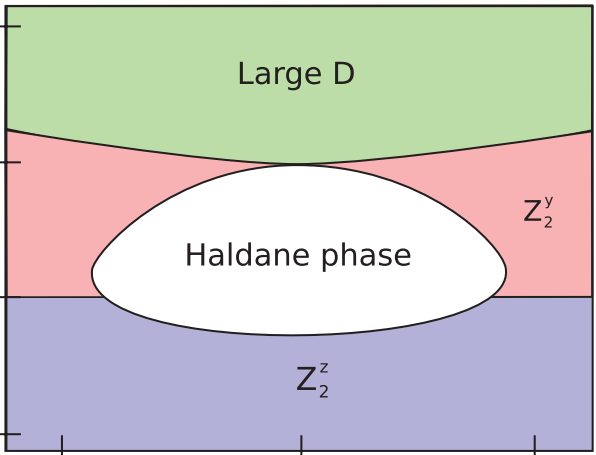
\includegraphics[width=\columnwidth]{diagrams/aklt2.png}
        \end{figure}
    \end{column}
    \begin{column}[T]{.55\textwidth}
    \vskip-0.8cm
    Two distinct featureless insulators:
    \bi 
    \item Large-D phase
    \bi 
    \item Contains product state wavefunction $\ket{\psi} = \ket{000...}$ 
    \ei
    \item Haldane phase
    \bi 
    \item Contains AKLT wavefunction $\ket{\psi} = \Sigma\ket{+00-0+...}$
    \ei 
        \begin{figure}[h]
            \hspace{-2cm}
            \scalebox{1.2}{
            \begin{frame}{MPS Example: AKLT State}
\vskip-1.5cm
\begin{block}{Haldane Phase for Spin-1 chains $(j=1, m=0)$}
\vskip-0.8cm
$$
H_{AKLT} = \sum\limits_{i} J \vec{S}_i\cdot \vec{S}_{i+1} + J' (\vec{S}_i\cdot \vec{S}_{i+1})^2 + D (S^z_i)^2+BS^x
$$
\end{block}
\begin{columns}[T]
    \begin{column}[T]{.45\textwidth}
        \vskip-1.2cm
        \begin{figure}
        \centering
        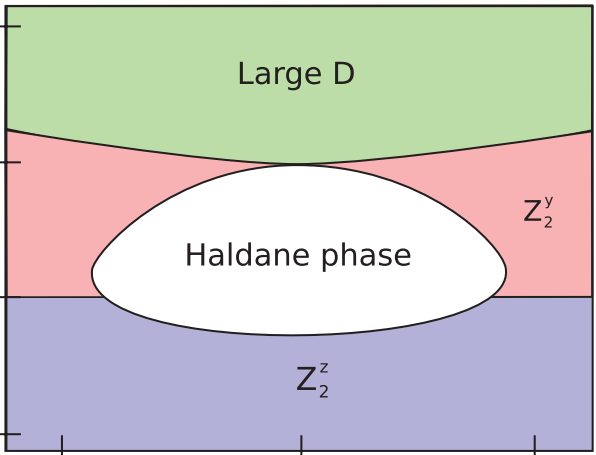
\includegraphics[width=\columnwidth]{diagrams/aklt2.png}
        \end{figure}
    \end{column}
    \begin{column}[T]{.55\textwidth}
    \vskip-0.8cm
    Two distinct featureless insulators:
    \bi 
    \item Large-D phase
    \bi 
    \item Contains product state wavefunction $\ket{\psi} = \ket{000...}$ 
    \ei
    \item Haldane phase
    \bi 
    \item Contains AKLT wavefunction $\ket{\psi} = \Sigma\ket{+00-0+...}$
    \ei 
        \begin{figure}[h]
            \hspace{-2cm}
            \scalebox{1.2}{
            \input{diagrams/aklt.tex}
            }
        \end{figure}

    \ei
    \end{column}
\end{columns}

\end{frame}
            }
        \end{figure}

    \ei
    \end{column}
\end{columns}

\end{frame}
            }
            \caption{Haldane phase of spin-1 Chain (AKLT)}
        \end{figure}
    \end{column}
\end{columns}
\end{frame}
\subsection{Lieb-Schultz-Mattis Theorem}
\begin{frame}{Lieb-Schultz-Mattis Theorem}
\vskip-1.5cm
 Featured states are 
 \bi 
 \item either gapless
 \item or spontaneously break spin symmetry
 \item or spontaneously break translational symmetry
 \item or topologically ordered
 \note{Why do we group these together? Shouldn't define a featureless insulator by what it is not.}
 \item {but always have (nearly) degenerate states when placed in periodic boundary conditions.}
 \ei 
 \note{This is a meaningful distinction because of the LSM}
 States with fractional charge per unit cell cannot be featureless.
\only<1>{
\begin{LSM}
A spin $1/2$ chain with $SU(2)$ and translational symmetry has a ground state that is either gapless or breaks symmetry.
\end{LSM}
}
\only<2>{
\begin{Oshikawa}
A particle-number conserving system with a fractional number of particles per unit cell cannot have a fixed energy gap on a torus.
The same holds for a $U(1)$-symmetric spin system with total spin $j$ per unit cell and magnetization $m$ per unit cell, with $j-m$ not integer. 
\end{Oshikawa}
}
\note{The argument for this is called the }
\only<3>{
\begin{block}{Proof:}
\begin{columns}[T]
\begin{column}[T]{0.6\textwidth}
{\em
The Lieb-Schultz-Mattis-Laughlin-Bonesteel-Affleck-Yamanaka-Oshikawa flux-threading argument}
\end{column}
\begin{column}[T]{0.4\textwidth}
\vskip-1.8cm
\begin{figure}
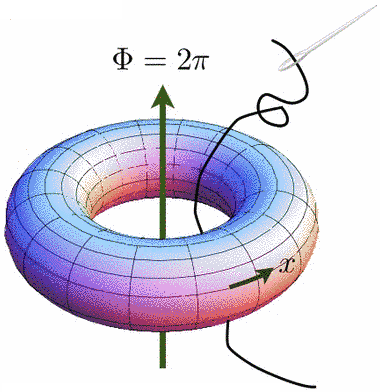
\includegraphics[width=0.9\columnwidth]{diagrams/flux-threading.png}
\end{figure}
\end{column}
\end{columns}
\end{block}
}
\end{frame}
\subsection{Magnetization Plateaus}
\begin{frame}{Application of LSM}
\vskip-1.5cm
\begin{block}{Spin-$1/2$ XXZ chain}
    \only<1>{
    \begin{equation*}
    H_{XY} = J \sum\limits_{i} (S^x_i S^x_{i+1} + S^y_i S^y_{i+1})
    \end{equation*}
    }
    \only<2>{
    \begin{equation*}
    H_{XY} = J \sum\limits_{i} (S^x_i S^x_{i+1} + S^y_i S^y_{i+1}+\frac{h}{J}S^z_i)
    \end{equation*}
    }
    \only<3>{
    \begin{equation*}
    H_{XXZ} = J \sum\limits_{i} (S^x_i S^x_{i+1} + S^y_i S^y_{i+1}+\Delta S^z_i S^z_{i+1} )
    \end{equation*}
    }
    \only<4>{
    \begin{equation*}
    H_{XXZ} = J \sum\limits_{i} (S^x_i S^x_{i+1} + S^y_i S^y_{i+1}+S^z_i S^z_{i+1}+\frac{J_2}{J}\vec{S}_i \cdot \vec{S}_{i+1})
    \end{equation*}
    }
Jordan-Wigner transformation maps to half-filled free-fermion band.
Remains gapless under small $U(1)$ perserving pertubations:
\end{block}
\begin{columns}[T]
    \begin{column}[T]{.53\textwidth}
        \bi
        \item<2-> $h S^z$ - gapless until $m=\pm 1/2$
        \item<3-> $J_z S^z_i S^z_{i+1}$ - gapless until AFM/FM order
        \item<4-> $J_2 \vec{S}_i \cdot \vec{S}_{i+2}$ - gapless until SSB of translation, unit cell doubles
        \ei 
    \end{column}
    \begin{column}[T]{.47\textwidth}
        \only<2>{
        \begin{figure}
            \centering
            \scalebox{0.6}{
            \begin{tikzpicture}
\tikzstyle{myedgestyle} = [-triangle 90]
\node[inv](A) at (0, -2){};
\node[inv](B) at (0, 2){};
\draw[thick, myedgestyle] (A)--node[left] {\huge $h$}(B);
\node[] at (3, -1.5){\LARGE Band metal};
\node[] at (3, 1.5){\LARGE Band insulator};
\draw[] (0.5, 0) -- (5.5, 0);
\end{tikzpicture}
            }
        \end{figure}
        }
        \only<3>{
            \vskip1.5cm
            \hspace{-0.8cm}
        \begin{figure}
            \centering
            \scalebox{0.47}{
            \begin{tikzpicture}
\tikzstyle{myedgestyle} = [triangle 90-triangle 90]
\node[inv](A) at (-6, 0){};
\node[inv](B) at (6, 0){};
\draw[thick, myedgestyle] (A)--node[below] {\huge $\Delta$}(B);
\node[] at (-5, 1.1){\LARGE  Gapped};
\node[] at (-5, 0.5){\LARGE  FM};
\node[] at (5, 1.1){\LARGE  Gapped};
\node[] at (5, 0.5){\LARGE  AFM};
\node[] at (0, 1.1){\LARGE  Gapless};
\node[] at (0, 0.5){\LARGE  XY phase};
\draw[] (-3,0) -- (-3,1.5);
\node[] at (-3, -0.5) {\LARGE $-1$};
\node[] at (3, -0.5) {\LARGE $+1$};
\draw[] (3,0) -- (3,1.5);
\end{tikzpicture}
            }
        \end{figure}
        }
        \only<4>{
        \begin{figure}
            \centering
            \scalebox{0.6}{
            \begin{tikzpicture}
\tikzstyle{myedgestyle} = [-triangle 90]
\node[inv](A) at (0, -2){};
\node[inv](B) at (0, 2){};
\draw[thick, myedgestyle] (A)--node[left] {\huge $J_2$}(B);
\node[] at (3, -1.5){\LARGE Gapless};
\node[] at (3, 1.5){\LARGE Dimerized};
\draw[] (0.5, 0) -- (5.5, 0);
\end{tikzpicture}
            }
        \end{figure}
        }
    \end{column}
    % \begin{column}[T]{.3\textwidth}
    % \end{column}
\end{columns}
% \begin{block}{Spin-$1$ Haldane Phase}
    % \begin{equation*}
    % H_{AKLT} = J \sum\limits_{i} (\vec{S}_i \cdot \vec{S}_{i+1})
    % \end{equation*}
% \end{block}
\end{frame}
\note{Now lets talk about the physics of some common featureless phases}
\begin{frame}{Magnetization/Density Plateaus}
\vskip-1.5cm
Stable featureless insulators form magnetization or density plateaus

Example Hamiltonians and phase diagrams:
\only<1>{
\begin{block}{Band Insulators}
\vskip-0.5cm
$$
H_{FF} =  \sum\limits_{<ij>}-t_{ij} c^{\dagger}_i c_j - \mu \sum\limits_i N_i 
$$
\end{block}
\begin{columns}[T]
    \begin{column}[T]{.45\textwidth}
        \vskip-1cm
        \begin{figure}
        \centering
        \scalebox{0.7}{
         \begin{tikzpicture}[domain=0:6.28]
      \draw[very thick] (0, -2.5) -- (0,1) node[left, midway] {\LARGE $E$} ;
      \draw[very thick] (0, 1)-- (6.28,1) -- (6.28, -2.5) -- (0, -2.5);
      \draw[color=black, very thick] plot (\x,{-1+cos(\x r)}) node[right] {};
      \draw[color=orange, fill] plot (\x,{-0.95+cos(\x r)}) {};
  \end{tikzpicture}
  
        }
        \end{figure}
    \end{column}
    \begin{column}[T]{.55\textwidth}
    \vskip-0.7cm
    \bi 
    \item Symmetry protected band touchings can constrain existence of a band insulator
    \note{beyond integer filling LSM, on a given lattice tight-bonding model}
    \item Topological invariants can distinguish different types of band insulators
    \item Some invariants only make sense in the presence of additional symmetries ($\mathcal{T}, \mathcal{C}, \mathcal{I}$)
    \ei
    \end{column}
\end{columns}
}
\only<2>{
\begin{block}{Bose-Hubbard model}
\vskip-0.5cm
$$
H_{BH} = -J \sum\limits_{<ij>} b^{\dagger}_i b_j - \mu \sum\limits_i N_i + \frac12 V \sum\limits_i N_i (N_i-1)
$$
\end{block}
\begin{columns}[T]
    \begin{column}[T]{.45\textwidth}
        \vskip-1.2cm
        \begin{figure}
        \centering
        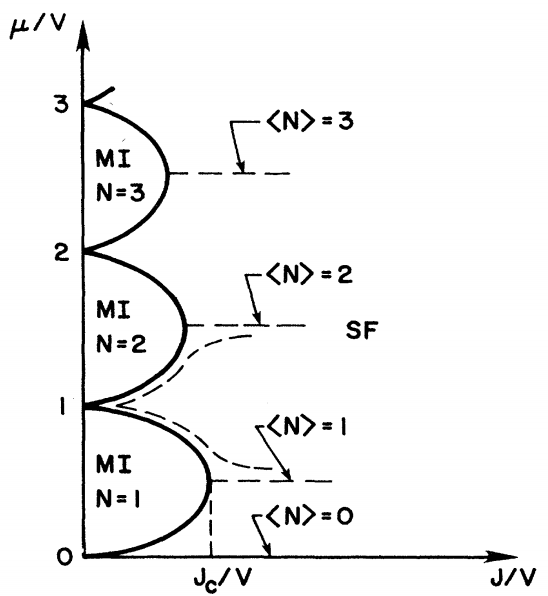
\includegraphics[width=4.5cm]{diagrams/bosehubbard2.png}
        \end{figure}
    \end{column}
    \begin{column}[T]{.55\textwidth}
    \vskip-0.7cm
    \bi 
    \item Interactions are always needed to stop Bose condensation
    \item Unlike free-fermions, not obvious how to construct fractional site filling insulators
    \item Tensor network states give us access to needed construction and to interacting invariants.
    \note{LSM inspired invariants}
    \ei
    \end{column}
\end{columns}
}

\only<3>{
\begin{block}{Haldane Phase for Spin-1 chains $(j=1, m=0)$}
\vskip-0.8cm
$$
H_{AKLT} = \sum\limits_{i} J \vec{S}_i\cdot \vec{S}_{i+1} + J' (\vec{S}_i\cdot \vec{S}_{i+1})^2 + D (S^z_i)^2+BS^x
$$
\end{block}
\begin{columns}[T]
    \begin{column}[T]{.45\textwidth}
        \vskip-1.2cm
        \begin{figure}
        \centering
        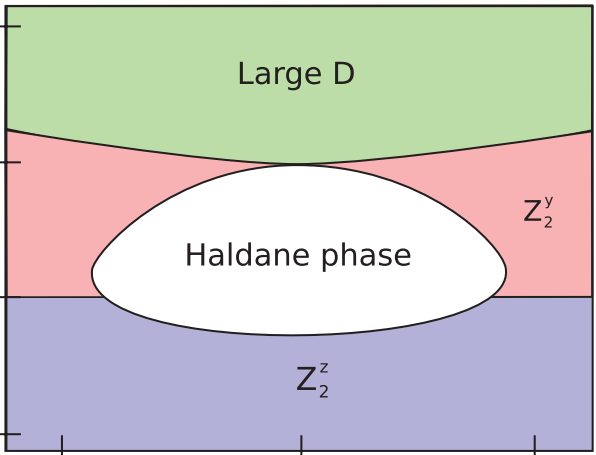
\includegraphics[width=\columnwidth]{diagrams/aklt2.png}
        \end{figure}
    \end{column}
    \begin{column}[T]{.55\textwidth}
    \vskip-0.8cm
    Two distinct featureless insulators:
    \bi 
    \item Large-D phase
    \bi 
    \item Contains product state wavefunction $\ket{\psi} = \ket{000...}$ 
    \ei
    \item Haldane phase
    \bi 
    \item Contains AKLT wavefunction $\ket{\psi} = \Sigma\ket{+00-0+...}$
    \ei 
        \begin{figure}[h]
            \hspace{-2cm}
            \scalebox{1.2}{
            \begin{frame}{MPS Example: AKLT State}
\vskip-1.5cm
\begin{block}{Haldane Phase for Spin-1 chains $(j=1, m=0)$}
\vskip-0.8cm
$$
H_{AKLT} = \sum\limits_{i} J \vec{S}_i\cdot \vec{S}_{i+1} + J' (\vec{S}_i\cdot \vec{S}_{i+1})^2 + D (S^z_i)^2+BS^x
$$
\end{block}
\begin{columns}[T]
    \begin{column}[T]{.45\textwidth}
        \vskip-1.2cm
        \begin{figure}
        \centering
        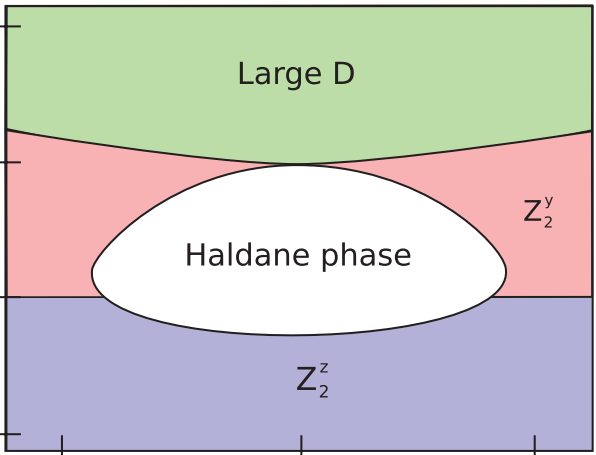
\includegraphics[width=\columnwidth]{diagrams/aklt2.png}
        \end{figure}
    \end{column}
    \begin{column}[T]{.55\textwidth}
    \vskip-0.8cm
    Two distinct featureless insulators:
    \bi 
    \item Large-D phase
    \bi 
    \item Contains product state wavefunction $\ket{\psi} = \ket{000...}$ 
    \ei
    \item Haldane phase
    \bi 
    \item Contains AKLT wavefunction $\ket{\psi} = \Sigma\ket{+00-0+...}$
    \ei 
        \begin{figure}[h]
            \hspace{-2cm}
            \scalebox{1.2}{
            \begin{frame}{MPS Example: AKLT State}
\vskip-1.5cm
\begin{block}{Haldane Phase for Spin-1 chains $(j=1, m=0)$}
\vskip-0.8cm
$$
H_{AKLT} = \sum\limits_{i} J \vec{S}_i\cdot \vec{S}_{i+1} + J' (\vec{S}_i\cdot \vec{S}_{i+1})^2 + D (S^z_i)^2+BS^x
$$
\end{block}
\begin{columns}[T]
    \begin{column}[T]{.45\textwidth}
        \vskip-1.2cm
        \begin{figure}
        \centering
        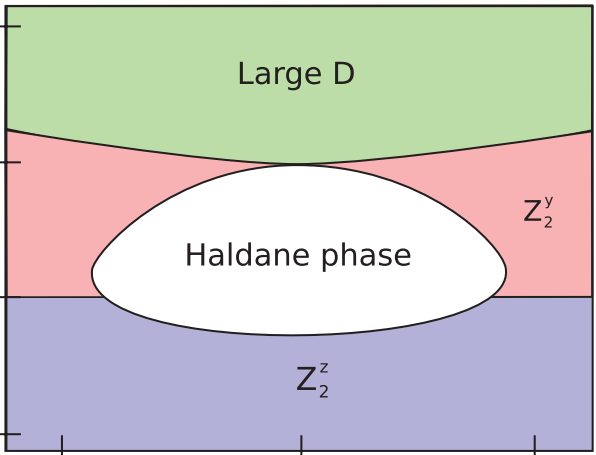
\includegraphics[width=\columnwidth]{diagrams/aklt2.png}
        \end{figure}
    \end{column}
    \begin{column}[T]{.55\textwidth}
    \vskip-0.8cm
    Two distinct featureless insulators:
    \bi 
    \item Large-D phase
    \bi 
    \item Contains product state wavefunction $\ket{\psi} = \ket{000...}$ 
    \ei
    \item Haldane phase
    \bi 
    \item Contains AKLT wavefunction $\ket{\psi} = \Sigma\ket{+00-0+...}$
    \ei 
        \begin{figure}[h]
            \hspace{-2cm}
            \scalebox{1.2}{
            \input{diagrams/aklt.tex}
            }
        \end{figure}

    \ei
    \end{column}
\end{columns}

\end{frame}
            }
        \end{figure}

    \ei
    \end{column}
\end{columns}

\end{frame}
            }
        \end{figure}

    \ei
    \end{column}
\end{columns}
}
% \only<3>{
% \bi
% \item Spin 3/2 Haldane Phase
% \ei
% $$
% H_{AKLT} = 
% $$
% \begin{figure}
% \centering
% \end{figure}
% }
\end{frame}
\begin{frame}{Motivating Questions}
\vskip -1.5cm

Are there general principles for distinguishing potential featureless insulator ground states of Hamiltonians?

The theory of {\em symmetry protected topological phases} (SPTs) is a general framework for distinguishing different featureless insulators.

\bi 
\item {\em Topological} - some discrete invariant that won't change under continuous (adiabatic) changes in Hamiltonian
\note{Can change when gap closes}
\item Invariants should be defined for interacting systems that obey certain symmetries 
\item Often features edge fractionalization and degeneracy in open boundary conditions
\item In 1D, universally distinguished by entanglement spectra
\ei

Are there additional constraints on the existence of featureless insulators in interacting systems?

\note{Any such constraint would be an extension of LSM}
\note{Those here who study topologically ordered states could care about this question because any such constraint lowers the burden of proof for T.O (only need to show gapped and symmetric.) (Of course, its still very hard to rule out symmetry breaking under complicated local order parameters or very large unit cells.)}
\note{Is this question at all related to the first question?}

\end{frame}
\section{Distinguishing Featureless Insulators by Entanglement}
\begin{frame}{What is entanglement?}
\vskip-1.5cm
 When a wavefunction in a product Hilbert space cannot be written as a product state, it is \textbf{entangled}.
\only<1-2>{ 
\begin{block}{}
\begin{columns}[T]
    \begin{column}{.5\textwidth}
    $$
    \ket{\psi} = \ket{\psi_L} \otimes \ket{\psi_R} ?
    $$
    \end{column}
    \begin{column}[T]{.5\textwidth}
        \only<1>{
        \note{A state in a product Hilbert space is a tensor}
        \vskip-1.5cm
        \begin{figure}
        \scalebox{0.8}
        {
        %!TEX root = ../thesis.tex

%\beginpgfgraphicnamed{diagrams}
\begin{tikzpicture}[node distance=0.4cm]
%\tikzset{ellip/.style={ellipse (3 and 1), fill=blue!20, draw=black, inner sep=4pt}}
\tikzset{det/.style={circle=2pt,fill=blue!20,draw=black,inner sep=4pt}}
%\draw (1,1) ellipse [x radius=1cm,y radius=.5cm];
\node[ellipse, rotate=0, draw, fill=blue!20] (t) at (0,0) {\, \, $\psi$ \, \,};
\node (t1) at (-1.6, 0.6) {$i_1$};
\node (t2) at (-1.2 ,0.85) {$i_2$};
\node (t3) at (-0.8,1.1) {$i_3$};
\node (t4) at (-0.3,1.2) {$i_4$};
\node (t5) at (0.3, 1.2) {$i_5$};
\node (tN) at (1.6, 0.6) {$i_N$};
\node[rotate=-20] (d) at (0.6, 0.6) {...};
%\node (tl) at (1,-0.4) {$l$};
\draw[thick] (t1) -- (t);
\draw[thick] (t2) -- (t);
\draw[thick] (t3) -- (t);
\draw[thick] (t4) -- (t);
\draw[thick] (t5) -- (t);

\draw[thick] (tN) -- (t);
%\node[in of=t] {$\psi$};
\node (p) at (0,-1) {$|\psi \rangle = \sum \psi_{i_1 i_2 ... i_N} \vert i_1 i_2 ... i_N \rangle$};


%\draw  (-0.8,2.4) node (v1) {} ellipse (1.2 and 0.4);
%\draw  (v1) ellipse (0 and 0);
\end{tikzpicture}
%\endpgfgraphicnamed
        }
        \end{figure}
        }
        \only<2>{
        \begin{figure}
        \vskip-1cm
        \scalebox{1}
        {
        \begin{tikzpicture}[node distance=0.6cm]
\node[side, minimum width=1cm] (psi) at (0,0) {$\psi$};
\node[above=of psi.north west, anchor=south west] (p) {};
\node[above=of psi.north east, anchor=south east] (q) {};
 \draw[->] (psi.north -| p) -- node[left] {$p$} (p);
 \draw[->] (psi.north -| q) -- node[right] {$q$} (q);
 
 \node at (1, 0) {=};
 
 \node[side] (psiL) at (1.8,0) {$\psi_L$};
  \node[side] (psiR) at (3.2,0) {$\psi_R$};
\node[above=of psiL.north west, anchor=south west] (pL) {};
\node[above=of psiR.north east, anchor=south east] (qR) {};
 \draw[->] (psiL.north -| pL) -- node[left] {$p$} (pL);
 \draw[->] (psiR.north -| qR) -- node[right] {$q$} (qR);
 
 
\end{tikzpicture}

% http://hugoideler.com/2013/01/tikz-node-positioning/
% \begin{tikzpicture}[
  % every node/.style={draw, minimum size=1cm, thick, fill=white, rounded corners},
  % hi/.style={fill=red!50},
  % low/.style={fill=blue!50},
% ]
  % \node[low, minimum width=5cm] (basis) {};
  % \node[hi, above=of basis.north west, anchor=south west] (a) {A};
  % \node[hi, above=of basis] (b) {B};
  % \node[hi, above=of basis.north east, anchor=south east] (c) {C};

  % \draw[->] (basis.north -| a) -- (a);
  % \draw[->] (basis) -- (b);
  % \draw[->] (basis.north -| c) -- (c);

  % \end{tikzpicture}
        }
        \note{going from the RHS to LHS - performing that sum - is tensor contraction. going from LHS to RHS is finding a decomposition of the tensor, and is not a unique process.}
        \end{figure}
        }
    \end{column}
\end{columns}
\end{block}
}
\only<3->{
\begin{block}{}
\begin{columns}[T]
    \begin{column}[T]{.5\textwidth}
    $$
    \ket{\psi} = \sum\limits_i \ket{\psi^i_L} \otimes \ket{\psi^i_R}
    $$
    \end{column}
    \begin{column}[T]{.5\textwidth}
        \begin{figure}
        \vskip-1cm
        \scalebox{1}
        {
        \begin{tikzpicture}[node distance=0.6cm]
\node[side, minimum width=1cm] (psi) at (0,0) {$\psi$};
\node[above=of psi.north west, anchor=south west] (p) {};
\node[above=of psi.north east, anchor=south east] (q) {};
 \draw[->] (psi.north -| p) -- node[left] {$p$} (p);
 \draw[->] (psi.north -| q) -- node[right] {$q$} (q);
 
 \node at (1, 0) {=};
 
 \node[side] (psiL) at (1.8,0) {$\psi_L$};
  \node[side] (psiR) at (3.2,0) {$\psi_R$};
\node[above=of psiL.north west, anchor=south west] (pL) {};
\node[above=of psiR.north east, anchor=south east] (qR) {};
 \draw[->] (psiL.north -| pL) -- node[left] {$p$} (pL);
 \draw[->] (psiR.north -| qR) -- node[right] {$q$} (qR);
 \draw[thick] (psiL) -- node[above] {$i$}(psiR);
 
\end{tikzpicture}

% http://hugoideler.com/2013/01/tikz-node-positioning/
% \begin{tikzpicture}[
  % every node/.style={draw, minimum size=1cm, thick, fill=white, rounded corners},
  % hi/.style={fill=red!50},
  % low/.style={fill=blue!50},
% ]
  % \node[low, minimum width=5cm] (basis) {};
  % \node[hi, above=of basis.north west, anchor=south west] (a) {A};
  % \node[hi, above=of basis] (b) {B};
  % \node[hi, above=of basis.north east, anchor=south east] (c) {C};

  % \draw[->] (basis.north -| a) -- (a);
  % \draw[->] (basis) -- (b);
  % \draw[->] (basis.north -| c) -- (c);

  % \end{tikzpicture}
        }
        \end{figure}
    \end{column}
\end{columns}
\end{block}
}
\only<3>{
\begin{block}{}
\vskip-0.5cm
Calculate reduced density matrices
\begin{columns}[T]
    \begin{column}[T]{.5\textwidth}
    $$
    \rho_L = Tr_R \ket{\psi} \bra{\psi} 
    $$
    
    \hskip0.3cm Diagonalize 
    
    $$
    \hskip0.1cm
    \rho_L = \sum\limits_{\alpha} \rho_{\alpha} \ket{\psi_L^{\alpha}} \bra{\psi_L^{\alpha}} 
    $$
    \end{column}
    \begin{column}[T]{.5\textwidth}
        \begin{figure}
        \vskip-0.5cm
        \scalebox{1}
        {
        \begin{tikzpicture}[node distance=0.6cm]
\node[side] (kL) at (0,0) {$\psi_L$};
\node[side] (kR) at (1.3, 0) {$\psi_R$};
\draw[thick] (kL) -- node[below] {$i$} (kR);
\node (kLp) at (0, 1) {};
\draw[thick] (kL) -- node[left] {$p$} (kLp);

\node[side] (bL) at (0,-1) {$\psi_L^*$};
\node[side] (bR) at (1.3, -1) {$\psi_R^*$};
\draw[thick] (bL) -- node[above] {$j$} (bR);
\node (bLp) at (0, -2) {};
\draw[thick] (bL) -- node[left] {$p'$} (bLp);

\node (kRp) at ($(kR.north)+(0.4, 0.4)$) {};
\node (bRp) at ($(bR.south)+(0.4, -0.4)$) {};
\draw[thick] (kR.north) to [bend left= 90] (kRp.center) to  [bend left=90] node[right] {$q$}  (bRp.center) to [bend left=90] (bR.south);


% \node[side] (UL) at (4, 0) {$U_S$};
% \node[side] (VL) at (5.4, 0) {$V_S$};
% \node[lambda] (SL) at (4.7, 0) {};
% \node[bel0w of=S] {$S_S$};

% \draw[thick] (UL) -- (SL) -- (VL);
% \node[side] (kL) at (4,0) {$\psi_S$};
% \node[side] (kR) at (7, 0) {$\psi_E$};
% \draw[thick] (VL) -- node[below] {$i$} (kR);
% \node (kLp) at (4, 1) {};
% \draw[thick] (UL) -- node[left] {$p_S$} (kLp);


% \node[side] (UdL) at (4, -1) {$U_S^*$};
% \node[side] (VdL) at (5.4, -1) {$V_S^*$};
% \node[lambda] (SdL) at (4.7, -1) {};
% \node[above of=SdL] {$S_S$};

% \draw[thick] (UdL) -- (SdL) -- (VdL);
% \node[side] (bR) at (7, -1) {$\psi_E^*$};
% \draw[thick] (VdL) -- node[above] {$j$} (bR);
% \node (bLp) at (4, -2) {};
% \draw[thick] (UdL) -- node[left] {$p'_S$} (bLp);

% \node (kRp) at ($(kR.north)+(0.4, 0.4)$) {};
% \node (bRp) at ($(bR.south)+(0.4, -0.4)$) {};
% \draw[thick] (kR.north) to [bend left= 90] (kRp.center) to  [bend left=90] node[right] {$p_E$}  (bRp.center) to [bend left=90] (bR.south);


\end{tikzpicture}
        }
        \end{figure}
    \end{column}
\end{columns}
\end{block}
}
\only<4->{
\begin{block}{}
\vskip-0.5cm
Diagonalize and form the Schmidt decomposition
\note{Equivalent to SVD}
\note{Schmidt states are orthonormal}
\begin{columns}[T]
    \begin{column}[T]{.5\textwidth}
    $$
    \ket{\psi} = \sum\limits_{\alpha} \sqrt{\rho_{\alpha}} \ket{\psi^{\alpha}_L} \otimes \ket{\psi^{\alpha}_R}
    $$
    \end{column}
    \begin{column}[T]{.5\textwidth}
        \begin{figure}
        \vskip-0.5cm
        \scalebox{1}
        {
        \begin{tikzpicture}[node distance=0.6cm]
\begin{scope}[decoration={
    markings,
    mark=at position 0.5 with {\arrow{>}}}
    ]
\node[side, minimum width=1cm] (psi) at (0,0) {$\psi$};
\node[above=of psi.north west, anchor=south west] (p) {};
\node[above=of psi.north east, anchor=south east] (q) {};
 \draw[->] (psi.north -| p) -- node[left] {$p$} (p);
 \draw[->] (psi.north -| q) -- node[right] {$q$} (q);
 
 \node at (1, 0) {=};
 
 \node[cside] (psiL) at (1.8,0) {$\psi_L$};
\node[lambda] (S) at (3, 0) {};
  \node[cside] (psiR) at (4.2,0) {$\psi_R$};
\node[above=of psiL.north west, anchor=south west] (pL) {};
\node[above=of psiR.north east, anchor=south east] (qR) {};
 \draw[->] (psiL.north -| pL) -- node[left] {$p$} (pL);
 \draw[->] (psiR.north -| qR) -- node[right] {$q$} (qR);
 \draw[-, postaction={decorate}] (S) -- node[above]{$\alpha$}(psiL);
 \draw[-, postaction={decorate}] (S) -- node[above]{$\alpha$}(psiR);
 
\end{scope}
\end{tikzpicture}
        }
        \end{figure}
    \end{column}
\end{columns}
\end{block}
\begin{block}{}
\vskip-0.5cm
\only<4>{
Quantitative measures of entanglement - rank
 $$
 S^0_A = \sum\limits_{\alpha} \rho_{\alpha}^0 = \#\{\rho_{\alpha} \ne 0\}
 $$
 \note{bond dimension}
 }
\only<5>{
Quantitative measures of entanglement - entropy
 $$
 S_A = -\sum\limits_{\alpha} \rho_{\alpha} \log{\rho_{\alpha} }
 $$
 \note{Capture MOST of the entanglement by using the largest eigenvalues, gives best possible approximation for a given bond dimension} 
 }
\end{block}
}

\end{frame}


\subsection{Matrix Product States}
\begin{frame}{What is a matrix product state?}
\vskip-1.5cm
Matrix product states provide a parameterization of the space of wavefunctions of a 1D or quasi-1D system.
\only<1, 3->{
\begin{figure}[h]
    \centering
    \scalebox{1}{
    \begin{tikzpicture}[node distance=0.4cm]
\tikzset{gamma/.style={circle=2pt,draw=black!100, very thick, fill=blue!40, inner sep=3pt}}


\begin{scope}[decoration={
    markings,
    mark=at position 0.5 with {\arrow{>}}}
    ]

\foreach \i in {1,...,6} {
	\node[gamma] (G\i) at (1.5*\i,0) {$A$};
	\node (l\i) at ($ (G\i) + (0, 1) $) {$$};
	\draw[very thick, red!100, postaction={decorate}] (G\i) -- (l\i);
	%\node[below of=G\i] {$A$};
}

\foreach \i in {7} {
	\node[] (G\i) at (1.5*\i,0) {$...$};
    }  
    
\foreach \i / \j in {1/2,2/3,3/4,4/5,5/6, 6/7} {
	\draw[very thick, postaction={decorate}] (G\j) -- (G\i);
}
\node (b0) at (0, 0) {$...$};
\draw[very thick, postaction={decorate}] (G1) -- (b0);

\end{scope}
\end{tikzpicture}

    }
\end{figure}
\only<1>{
$$
\ket{\psi^{b_0 b_1}} = \sum\limits_{p_1 ... p_5}   \vbra{b_0} A^{p_1}_1 ... A^{p_5}_5 \vket{b_1}\ket{p_1 ... p_5} 
$$
}
Coefficients of the wavefunction are calculated via a product of matrices, one per site. The matrix at each site depends on the physical state at that site.
}

\only<2>{
\begin{figure}[h]
    \centering
    \scalebox{1}{
    \begin{tikzpicture}[node distance=0.4cm]
\begin{scope}[decoration={
    markings,
    mark=at position 0.5 with {\arrow{>}}}
    ]
\foreach \i in {1,...,5} {
	\node[gamma] (G\i) at (1.5*\i,0) {};
	\node (l\i) at ($ (G\i) + (0, 1) $) {$p_\i$};
	\draw[thick] (G\i) -- (l\i);
	\node[below of=G\i] {$A^\i$};
}
\foreach \i / \j in {1/2,2/3,3/4,4/5} {
	\draw[thick, postaction={decorate}] (G\j) -- (G\i);
}
\node[side] (B) at (0.5, 0) {$B$};
%\node (b1) at (0, 0) {$b_1$};
\draw[thick, postaction={decorate}] (G1) -- node[below]{$b_0$}(B);
\draw[thick, postaction={decorate}] (8.1, 0)--(G5.east);
\draw[thick, postaction={decorate}] (B.west) -- node[below]{$b_1$}(-0.1, 0);
\end{scope}
\draw[thick, dashed] (0.2,0) .. controls (-1,0) and (-0.6,0.6) .. (4,0.5) .. controls (8.5,0.5) and (9,0) .. (7.5,0);
\end{tikzpicture}
    }
\end{figure}

\only<2>{
$$
\ket{\psi} = \sum\limits_{p_1 ... p_5}   Tr(B A^{p_1}_1 ... A^{p_5}_5)\ket{p_1 ... p_5} 
$$
}

}
\only<3->{
Every state has a matrix product state representation formed through the process of repeated SVD.

\only<3>{
\begin{figure}[h]
    \centering
    \scalebox{1.1}{
    \begin{tikzpicture}[node distance=0.6cm]

\node[side, minimum width=1.6cm, minimum height=0.8cm] (psi) at (0,0) {$\psi$};
\node[above=of psi.north west, anchor=south west] (p1) {};
\node[above=of psi](p2) {};
\node[above=of psi.north east, anchor=south east] (p3) {};
\node at (1.3, 0) {=}; 
\node[cside] (psi1) at (2.2,0) {$U_1$};
\node[lambda] (S) at (3.4, 0) {};
\node[cside] (psiR) at (4.8,0) {$V_1$};
\node[above=of psi1.north west, anchor=south west] (pL) {};
\node[above=of psiR.north west, anchor=south west] (q2) {};
\node[above=of psiR.north east, anchor=south east] (qR) {};

\begin{scope}[decoration={
    markings,
    mark=at position 0.5 with {\arrow{>}}}
    ]
 \draw[->] (psi.north -| p1) -- node[left] {$p_1$} (p1);
 \draw[->] (psi) --  node[left] {$p_2$} (p2);
 \draw[->] (psi.north -| p3) -- node[left] {$p_3$} (p3);
 \draw[->] (psi1.north -| pL) -- node[left] {$p_1$} (pL);
 \draw[->] (psiR.north-|q2)-- node[left] {$p_2$} (q2);
 \draw[->] (psiR.north -| qR) -- node[right] {$p_3$} (qR);
 \draw[-, thick, postaction={decorate}]  (S) -- (psi1);
 \draw[-, thick, postaction={decorate}] (S) -- (psiR);
 \end{scope}
 \end{tikzpicture}
    }
    \note{Maximum bond dimension d}
\end{figure}
}
\only<4>{
\begin{figure}[h]
    \centering
    \scalebox{1.1}{
    \begin{tikzpicture}[node distance=0.6cm]
    \node[side, minimum width=1.5cm, minimum height=0.8cm] (psi) at (0,0) {$\psi$};
    \node[above=of psi.north west, anchor=south west] (p1) {};
    \node[above=of psi](p2) {};
    \node[above=of psi.north east, anchor=south east] (p3) {};
    \node at (1.3, 0) {=}; 
    \node[cside] (psi1) at (2,0) {$U_1$};
    %\node[lambda] (S) at (3, 0) {};
    \node[side,minimum width=1cm, minimum height=0.8cm] (psiR) at (4.2,0) {$\psi'$};
    \node[above=of psi1.north west, anchor=south west] (pL) {};
    \node[above=of psiR.north west, anchor=south west] (q2) {};
    \node[above=of psiR.north east, anchor=south east] (qR) {};
\begin{scope}[decoration={
    markings,
    mark=at position 0.5 with {\arrow{>}}}
    ]
    \draw[->] (psi.north -| p1) -- node[left] {$p_1$} (p1);
    \draw[->] (psi) --  node[left] {$p_2$} (p2);
    \draw[->] (psi.north -| p3) -- node[left] {$p_3$} (p3);
    \draw[->] (psi1.north -| pL) -- node[left] {$p_1$} (pL);
    \draw[->] (psiR.north-|q2)-- node[left] {$p_2$} (q2);
    \draw[->] (psiR.north -| qR) -- node[right] {$p_3$} (qR);
    \draw[-, thick, postaction={decorate}] (psiR) -- node[above]{$i_1$}(psi1);
  \end{scope}
\end{tikzpicture}
    }
    \note{Maximum bond dimension d^2}
\end{figure}
}
\only<5>{
\begin{figure}[h]
    \centering
    \scalebox{1.1}{
    \begin{tikzpicture}[node distance=0.6cm]
    \node[side, minimum width=1.5cm, minimum height=0.8cm] (psi) at (0,0) {$\psi$};
    \node[above=of psi.north west, anchor=south west] (p1) {};
    \node[above=of psi](p2) {};
    \node[above=of psi.north east, anchor=south east] (p3) {};
    \node at (1.3, 0) {=};
    \node[cside] (B1) at (2,0) {$U_1$};
    \node[cside] (B2) at (3.5,0) {$U_2$};
    \node[side, minimum width=0.5cm, minimum height=0.8cm](psiR) at (5, 0){$\psi''$};
    %\node[lambda] (S) at (3, 0) {};
    %\node[side,minimum width=1cm, minimum height=0.8cm] (psiR) at (4.2,0) {$\psi'$};
    \node[above=of B1.north, anchor=south] (pL) {};
    \node[above=of B2] (q2) {};
    %\node[above=of psiR.north west, anchor=south west] (q2) {};
    \node[above=of psiR.north, anchor=south] (qR) {};
\begin{scope}[decoration={
    markings,
    mark=at position 0.5 with {\arrow{>}}}
    ]
    \draw[->] (psi.north -| p1) -- node[left] {$p_1$} (p1);
    \draw[->] (psi) --  node[left] {$p_2$} (p2);
    \draw[->] (psi.north -| p3) -- node[left] {$p_3$} (p3);
    \draw[->] (B1.north -| pL) -- node[left] {$p_1$} (pL);
    \draw[->] (B2.north-|q2)-- node[left] {$p_2$} (q2);
    \draw[->] (psiR.north -| qR) -- node[right] {$p_3$} (qR);
    \draw[-, thick, postaction={decorate}] (B2) -- node[above]{$i_1$}(B1);
    \draw[-, thick, postaction={decorate}] (psiR) -- node[above]{$i_2$}(B2);
 %\draw[-] (psiR) -- (S);
  \end{scope}
\end{tikzpicture}
    }
\end{figure}
}
}

\end{frame}
\begin{frame}{Tensor Network States}
\vskip-1.5cm
\begin{columns}[T]
\begin{column}[T]{.5\textwidth}
\bi
\item MPS and the generalization to PEPS automatically satisfy area law.

\item Entanglement rank and entropy bounded by total bond dimension across any cut.

\item Can view PEPS on cylinder as a MPS.
\ei 
\end{column}
\begin{column}{.5\textwidth}
\vskip-0.7cm
\begin{figure}
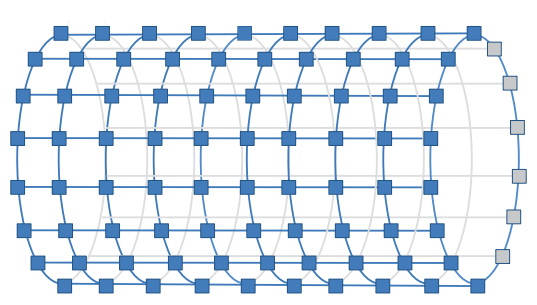
\includegraphics[width=6cm]{diagrams/CylPEPS1.png}
\caption{Translationally symmetric PEPS on a cylinder}
\end{figure}
\vskip-0.6cm
\begin{figure}
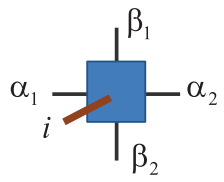
\includegraphics[width=2cm]{diagrams/CylPEPS2.png}
\caption{Close-up of site-tensor in PEPS}
\end{figure}
\end{column}
\end{columns}
\end{frame}
\begin{frame}{Computing Correlation Functions in MPS}
\vskip-1.5cm
\only<1,3->{
\begin{figure}[t]
\centering
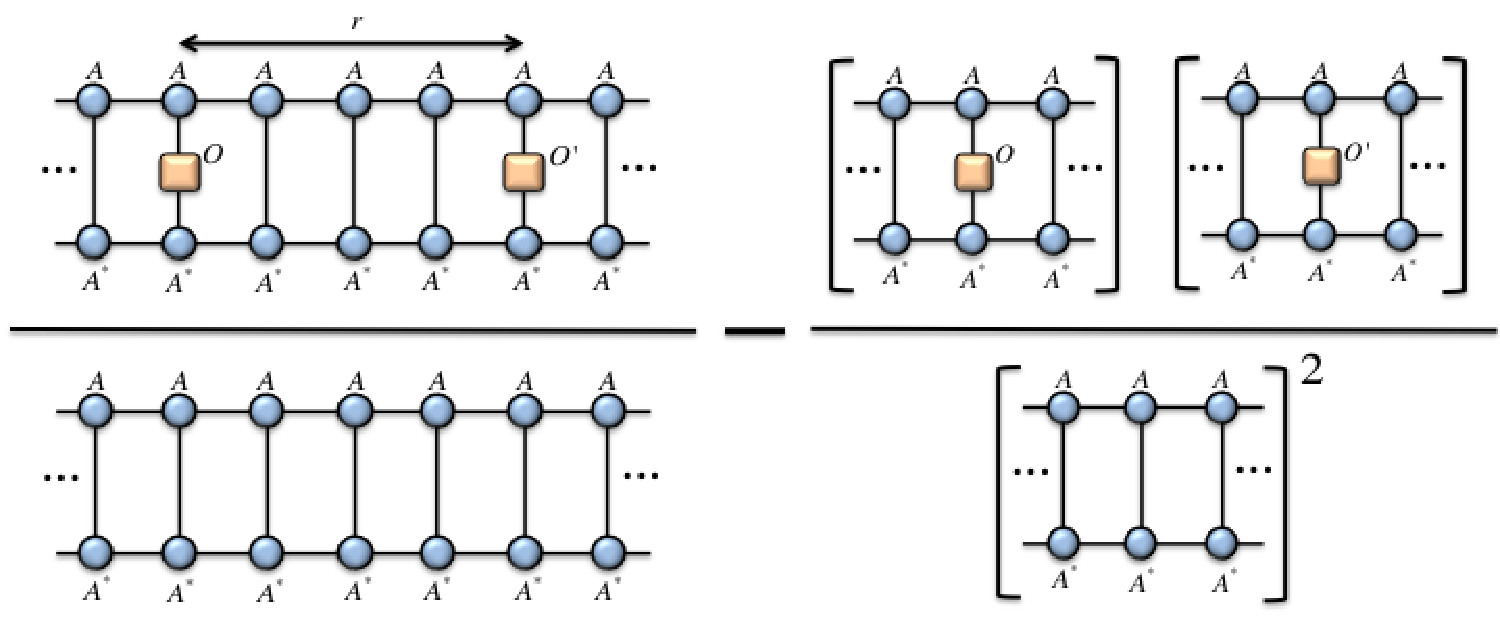
\includegraphics[width=\textwidth]{diagrams/orus-corrfunc.pdf}
%\begin{tikzpicture}[node distance=0.5cm]

\foreach \i in {1,...,5} {
	\node (Gp\i) at (1.5*\i,-2.5) [gamma] {};
	\node (Gpp\i) at ($ (Gp\i) + (0,-1) $) [gamma] {};
	\draw[thick] (Gp\i) -- (Gpp\i);
	\node[above of=Gp\i] {$A^\i$};
	\node[below of=Gpp\i] {$(A^\i)^*$};
}
\foreach \i / \j in {1/2,2/3,3/4,4/5} {
	\draw[thick] (Gp\i) -- (Gp\j);
	\draw[thick] (Gpp\i) -- (Gpp\j);
}

\foreach \i in {1,...,5} {
	\node (Gp\i) at (1.5*\i,-5.5) [gamma] {};
	\node (Gpp\i) at ($ (Gp\i) + (0,-2) $) [gamma] {};
	\node (O\i) at ($ (Gp\i) + (-0,-1) $) [operator] {};
	
	\draw[thick] (Gp\i) -- (O\i);
	\draw[thick] (Gpp\i) -- (O\i);
	
	\node[above of=Gp\i] {$A^\i$};
	\node[below of=Gpp\i] {$(A^\i)^*$};
	\node[above left of=O\i] {$W^\i$};
}
\foreach \i / \j in {1/2,2/3,3/4,4/5} {
	\draw[thick] (Gp\i) -- (Gp\j);
	\draw[thick] (Gpp\i) -- (Gpp\j);
	\draw[thick] (O\i) -- (O\j);
}

\end{tikzpicture}

\caption{Diagram for $C_{O O'}(r) = \ev{O_i O'_{i+r}}- \ev{O_i}\ev{O'_{i+r}}$}
\end{figure}
}
\only<2>{
\begin{columns}[T]
    \begin{column}[T]{.28\textwidth}
        \begin{figure}[h]
            \centering
            \scalebox{1}{
            \begin{tikzpicture}[node distance=0.4cm]
\begin{scope}[thick, decoration={
    markings,
    mark=at position 0.5 with {\arrow{>}}}
    ]
  \node[gamma] (A) at (0,0) {$A$};  
  \node[gamma] (Ac) at (0,2) {$A^{*}$};
  \draw[postaction={decorate}] (A)--(Ac);
  \node[inv] (ki) at (1, 0){};
  \node[inv] (bi) at (1, 2){}; 
  \node[inv] (ko) at (-1, 0){}; 
  \node[inv] (bo) at (-1, 2){};
  \draw[color=red, postaction={decorate}] (ki)--(A);
  \draw[color=green, postaction={decorate}] (bi)--(Ac);
  \draw[color=red, postaction={decorate}] (A) -- (ko);
  \draw[color=green, postaction={decorate}] (Ac) -- (bo);

\end{scope}
\end{tikzpicture}

            }
            \caption{Transfer Matrix $\mathbb{E}_{I}$}
            \note{Reminder using arrows to represent in and out}
        \end{figure}
    \end{column}
    \begin{column}[T]{.3\textwidth}
        \begin{figure}[h]
            \centering
            \scalebox{1}{
            \begin{tikzpicture}[node distance=0.4cm]
\begin{scope}[thick, decoration={
    markings,
    mark=at position 0.5 with {\arrow{>}}}
    ]
  \node[gamma] (A) at (0,0) {$A$};  
  \node[operator] (O) at (0, 1) {$O$};
 % \node[operator] (O2) at (0, 1) {$O'$};
  \node[gamma] (Ac) at (0,2) {$A^{*}$};
  \draw[postaction={decorate}] (A)-- (O) -- (Ac);
  \node[inv] (ki) at (1, 0){};
  \node[inv] (bi) at (1, 2){}; 
  \node[inv] (ko) at (-1, 0){}; 
  \node[inv] (bo) at (-1, 2){};
  \draw[color=red, postaction={decorate}] (ki)--(A);
  \draw[color=green, postaction={decorate}] (bi)--(Ac);
  \draw[color=red, postaction={decorate}] (A) -- (ko);
  \draw[color=green, postaction={decorate}] (Ac) -- (bo);

\end{scope}
\end{tikzpicture}
            }
            \caption{Operator Insertion $\mathbb{E}_{O}$}
        \end{figure}
    \end{column}
    \begin{column}[T]{.42\textwidth}
        \vskip1.8cm
        \begin{figure}[h]
            \centering
            \scalebox{0.8}{
            \begin{tikzpicture}
\begin{scope}[very thick,decoration={
    markings,
    mark=at position 0.5 with {\arrow{>}}}
    ] 

\node[peps] (A1) at (-4.1, 0) {};
\node (li) at ($(A1) + (-1, 0) $) {};
\draw[thick, postaction={decorate}] (li.center) -- (A1.west);
\draw[thick, postaction={decorate}] (A1.east) -- node[right] {} +(1,0);
\draw[thick, postaction={decorate}] (A1.north) -- node[above] {} +(0,0.5);

\node at (-2.3, 0.5){$= e^{i \theta}$};    

\node[peps] (A) at (0, 0) {};
\node[draw] (Ul) at ($(A) + (-1, 0) $) {$U$};
\node[draw] (Ur) at ($(A) + (1, 0) $) {$U^{\dagger}$};
\node (LI) at ($(Ul) + (-1, 0) $) {};
\draw[thick, postaction={decorate}] (LI.center) -- (Ul.west);
\draw[thick, postaction={decorate}] (Ur.east) -- node[right] {} +(0.5,0);
\draw[thick, postaction={decorate}] (Ul) -- (A);
\draw[thick, postaction={decorate}] (A) -- (Ur);
\draw[thick, postaction={decorate}] (A.north) -- node[above] {} +(0,0.5);

\end{scope}
\end{tikzpicture}
            }
            \caption{MPS gauge redundancy}
        \end{figure}
    \end{column}
\end{columns} 
\begin{figure}[h]
    \centering
    \scalebox{1}{
    \begin{tikzpicture}[node distance=0.4cm]
\begin{scope}[thick, decoration={
    markings,
    mark=at position 0.5 with {\arrow{>}}}
    ]
  \node[gamma] (A) at (0,0) {$A$};  
  \node[gamma] (Ac) at (0,2) {$A^{*}$};
  \node[side, minimum height=1.97cm] (vR) at (1.5, 1){$v_R$};
  \draw[postaction={decorate}] (A)--(Ac);
  \node[inv] (ki) at (1, 0){};
  \node[inv] (bi) at (1, 2){}; 
  \node[inv] (ko) at (-1, 0){}; 
  \node[inv] (bo) at (-1, 2){};
  \draw[color=red, postaction={decorate}] (vR.south west) -- (ki.center)--(A);
  \draw[color=green, postaction={decorate}] (vR.north west)-- (bi.center)--(Ac);
  \draw[color=red, postaction={decorate}] (A) -- (ko);
  \draw[color=green, postaction={decorate}] (Ac) -- (bo);
  
  \node[] at (2.5, 1){$=$};
  \node[side, minimum height=1.97cm] (vR) at (3.5, 1){$v_R$};
  \node[inv] (ki) at (2.5, 0){};
  \node[inv] (bi) at (2.5, 2){};
  \draw[color=red, postaction={decorate}] (vR.south west) -- (ki.center);
  \draw[color=green, postaction={decorate}] (vR.north west)-- (bi.center); 

  \node[] at (4.5, 1){$=$};
  \node[side, minimum height=0.6cm] (sR) at (5.5, 0){$\sigma_R$};
  \node[inv] (ki) at (4.5, 0){};
  \node[inv] (k2) at (6.3, 0){};
  \node[cdot] (dot) at (6.3, 1){};
   \node[inv] (b2) at (6.3, 2){};
  \node[inv] (bi) at (4.5, 2){};
  \draw[color=red, postaction={decorate}]  (dot)--(k2.center);
  \draw[color=red, postaction={decorate}]  (k2.center)-- (sR.east);
  \draw[color=red, postaction={decorate}]  (sR.west) -- (ki.center);
  \draw[color=green, postaction={decorate}]  (dot)--(b2.center);
  \draw[color=green, postaction={decorate}]  (b2.center)-- (bi);
\end{scope}
\end{tikzpicture}
    }
\caption{Eigenvector equation $\mathbb{E}_{I}(\sigma_R) = \sigma_R$}
\end{figure}
   
}
\only<3>{
\vskip-0.5cm
 $$\ev{O_i O'_{i+r}} = \vbraopket{v_L}{\mathbb{E}_O \mathbb{E}_I^r \mathbb{E}_{O'}}{v_R}$$
 $$
 \lim\limits_{r \rightarrow \infty} \ev{O_i O'_{i+r}} = \vbraopket{v_L}{\mathbb{E}_O}{v_R} \vbraopket{v_L}{\mathbb{E}_{O'}}{v_R}
 $$
 $$ C_{O O'}(r) \approx const. \times \lambda_2^r $$
\note{Matrix product states also known as finitely correlated states}
}
\end{frame}
\begin{frame}{Computing Entanglement in MPS/PEPS}
\vskip-1.5cm
To compute the spectrum of the reduced density matrix 
\only<1, 2>{
\begin{figure}
\scalebox{1}{
            \begin{tikzpicture}[node distance=0.4cm]
\begin{scope}[decoration={
    markings,
    mark=at position 0.5 with {\arrow{>}}}
    ]
\node[] (rho) at (-0.5,1) {\Large $\rho =$};      
\foreach \i in {1,...,3} {
	\node[gamma] (G\i) at (1.5*\i,0) {$A$};
	\node (l\i) at ($ (G\i) + (0, 1) $) {$$};
	\draw[thick, postaction={decorate}] (G\i) -- (l\i);
	%\node[below of=G\i] {$A$};
}
\foreach \i / \j in {1/2,2/3} {
	\draw[thick, postaction={decorate}] (G\j) -- (G\i);
}
\node (b0) at (0, 0) {$...$};
\draw[thick, postaction={decorate}] (G1) -- (b0);

\foreach \i in {1,...,3} {
	\node[gamma] (B\i) at (1.5*\i,2) {$A^*$};
	\node (l\i) at ($ (B\i) + (0, -1) $) {$$};
	\draw[thick, postaction={decorate}] (l\i) -- (B\i);
	%\node[below of=G\i] {$A$};
}
\foreach \i / \j in {1/2,2/3} {
	\draw[thick, postaction={decorate}] (B\i) -- (B\j);
}
\node (b1) at (0, 2) {$...$};
\draw[thick, postaction={decorate}] (b1) -- (B1);

\foreach \i in {4,...,6} {
	\node[gamma] (G\i) at (1.5*\i,0) {$A$};
	\node[gamma] (B\i) at (1.5*\i,2) {$A^*$};
	\draw[thick, postaction={decorate}] (G\i) -- (B\i);
	}
\foreach \i in {7} {
	\node[] (G\i) at (1.5*\i,0) {$...$};
	\node[] (B\i) at (1.5*\i,2) {$...$};
    }  
\foreach \i / \j in {3/4,4/5,5/6, 6/7} {
	\draw[thick, postaction={decorate}] (G\j) -- (G\i);
	\draw[thick, postaction={decorate}] (B\i) -- (B\j);
}
\end{scope}
\end{tikzpicture}

            }
\end{figure}
}

\only<3>{
\begin{figure}
\scalebox{1}{
            \begin{tikzpicture}[node distance=0.4cm]
\begin{scope}[decoration={
    markings,
    mark=at position 0.5 with {\arrow{>}}}
    ]
\node[] (rho) at (4.5,1) {\Large $\widetilde{\rho} =$};  

\foreach \i in {3} {
	\node[inv] (G\i) at (1.5*\i,0) {$A$};
	\node[inv] (B\i) at (1.5*\i,2) {$A^*$};
    }
\foreach \i in {7} {
	\node[] (G\i) at (1.5*\i,0) {$...$};
	\node[] (B\i) at (1.5*\i,2) {$...$};
    }    
\foreach \i in {4,...,6} {
	\node[gamma] (G\i) at (1.5*\i,0) {$A$};
	\node[gamma] (B\i) at (1.5*\i,2) {$A^*$};
	\draw[thick, postaction={decorate}] (G\i) -- (B\i);
	}
\foreach \i / \j in {3/4,4/5,5/6, 6/7} {
	\draw[thick, postaction={decorate}] (G\j) -- (G\i);
	\draw[thick, postaction={decorate}] (B\i) -- (B\j);
}
\end{scope}
\end{tikzpicture}

            }
\end{figure}
}
\only<2>{
A valid simplified case is when the contraction 
\begin{figure}
\scalebox{1}{
            \begin{tikzpicture}[node distance=0.4cm]
\begin{scope}[decoration={
    markings,
    mark=at position 0.5 with {\arrow{>}}}
    ]
\node[] (u) at (-0.5, 0) {\Large $\mathcal{U} =$}; 
\foreach \i in {1,...,3} {
	\node[gamma] (G\i) at (1.5*\i,0) {$A$};
	\node (l\i) at ($ (G\i) + (0, 1) $) {$$};
	\draw[thick, postaction={decorate}] (G\i) -- (l\i);
	%\node[below of=G\i] {$A$};
}
\foreach \i / \j in {1/2,2/3} {
	\draw[thick, postaction={decorate}] (G\j) -- (G\i);
}
\node (b0) at (0, 0) {$...$};
\node[inv] (sigL) at (6, 0) {$\frac{1}{\sqrt{\sigma_L}}$};
\draw[thick, postaction={decorate}] (G1) -- (b0);
\draw[thick, postaction={decorate}] (sigL) -- (G3);
%\node[inv](Q) at (7, 0){};
%\draw[thick, postaction={decorate}] (Q) -- (sigL);
\end{scope}
\end{tikzpicture}

            }
\end{figure}

is isometric. We can always get into this canonical form.
}


\only<3>{
\bi 
\item $\rho = \mathcal{U} \cdot \widetilde{\rho} \cdot \mathcal{U}^{\dagger}$
\item $\widetilde{\rho}$ is isometric to real $\rho$ - same spectrum, many less 0s.
\ei
}
\end{frame}
\begin{frame}{MPS Example: AKLT State}
\vskip-1.5cm
\begin{figure}
\scalebox{2}{
            \begin{frame}{MPS Example: AKLT State}
\vskip-1.5cm
\begin{block}{Haldane Phase for Spin-1 chains $(j=1, m=0)$}
\vskip-0.8cm
$$
H_{AKLT} = \sum\limits_{i} J \vec{S}_i\cdot \vec{S}_{i+1} + J' (\vec{S}_i\cdot \vec{S}_{i+1})^2 + D (S^z_i)^2+BS^x
$$
\end{block}
\begin{columns}[T]
    \begin{column}[T]{.45\textwidth}
        \vskip-1.2cm
        \begin{figure}
        \centering
        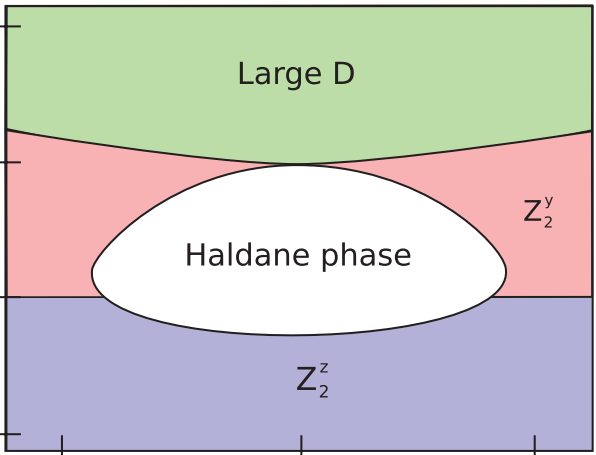
\includegraphics[width=\columnwidth]{diagrams/aklt2.png}
        \end{figure}
    \end{column}
    \begin{column}[T]{.55\textwidth}
    \vskip-0.8cm
    Two distinct featureless insulators:
    \bi 
    \item Large-D phase
    \bi 
    \item Contains product state wavefunction $\ket{\psi} = \ket{000...}$ 
    \ei
    \item Haldane phase
    \bi 
    \item Contains AKLT wavefunction $\ket{\psi} = \Sigma\ket{+00-0+...}$
    \ei 
        \begin{figure}[h]
            \hspace{-2cm}
            \scalebox{1.2}{
            \begin{frame}{MPS Example: AKLT State}
\vskip-1.5cm
\begin{block}{Haldane Phase for Spin-1 chains $(j=1, m=0)$}
\vskip-0.8cm
$$
H_{AKLT} = \sum\limits_{i} J \vec{S}_i\cdot \vec{S}_{i+1} + J' (\vec{S}_i\cdot \vec{S}_{i+1})^2 + D (S^z_i)^2+BS^x
$$
\end{block}
\begin{columns}[T]
    \begin{column}[T]{.45\textwidth}
        \vskip-1.2cm
        \begin{figure}
        \centering
        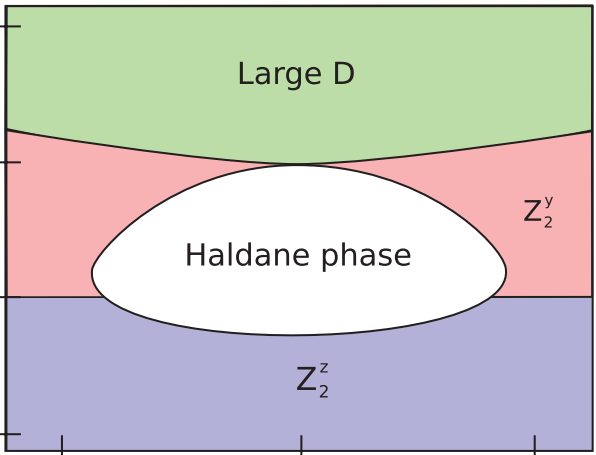
\includegraphics[width=\columnwidth]{diagrams/aklt2.png}
        \end{figure}
    \end{column}
    \begin{column}[T]{.55\textwidth}
    \vskip-0.8cm
    Two distinct featureless insulators:
    \bi 
    \item Large-D phase
    \bi 
    \item Contains product state wavefunction $\ket{\psi} = \ket{000...}$ 
    \ei
    \item Haldane phase
    \bi 
    \item Contains AKLT wavefunction $\ket{\psi} = \Sigma\ket{+00-0+...}$
    \ei 
        \begin{figure}[h]
            \hspace{-2cm}
            \scalebox{1.2}{
            \input{diagrams/aklt.tex}
            }
        \end{figure}

    \ei
    \end{column}
\end{columns}

\end{frame}
            }
        \end{figure}

    \ei
    \end{column}
\end{columns}

\end{frame}
            }
\end{figure}
\begin{columns}[T]
\begin{column}[T]{.5\textwidth}
\vskip-1.5cm
\begin{figure}
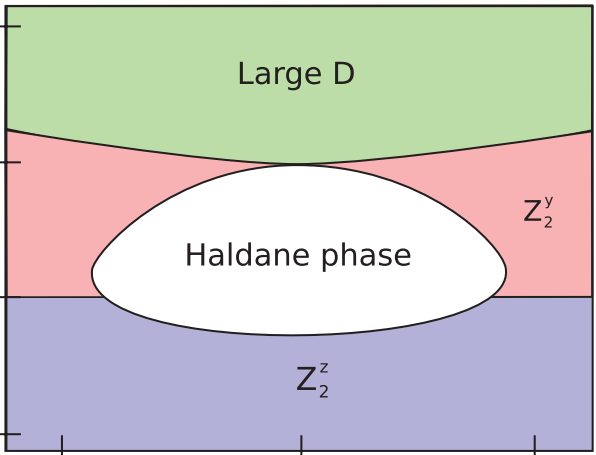
\includegraphics[width=\columnwidth]{diagrams/aklt2.png}
\end{figure}
\end{column}
   \begin{column}[T]{.5\textwidth}
   \vskip-1cm
    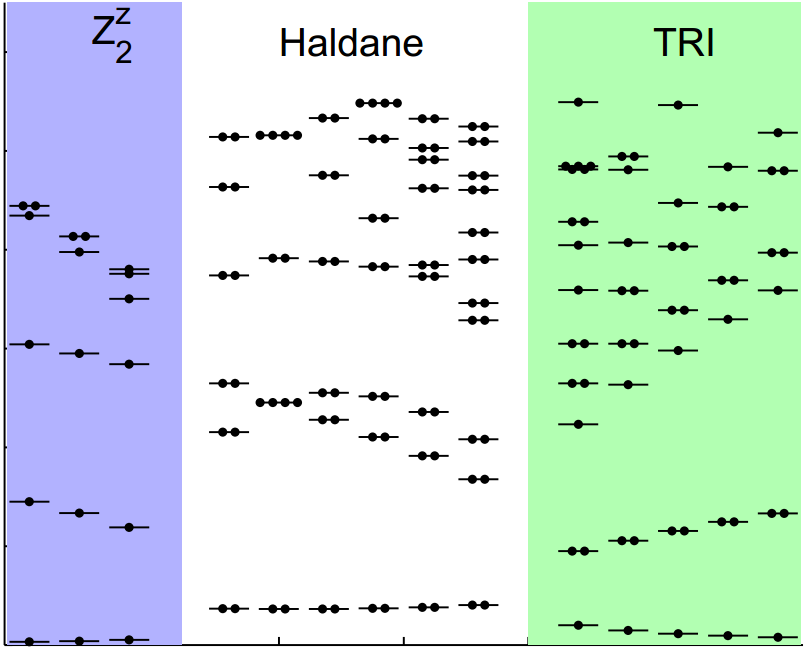
\includegraphics[width=\columnwidth]{diagrams/akltEE.png}
    \end{column}
\end{columns}

Haldane phase distinguished by exact double degeneracy in entire  entanglement spectrum.
\end{frame}
\begin{frame}{Properties of Featureless MPS}
\vskip-1.5cm
MPS for featureless 1D or quasi-1D systems have non-degenerate transfer matrices and are called simple. Simple MPS can be proved to have:

\bi 
\item Correlations are insensitive to boundary conditions
\item Can construct a featureless 'parent Hamiltonian' 
\note{from the wavefunction alone}
\item Two simple MPS with equal wavefunctions are (uniquely) gauge equivalent
\item Corollary: Edges can be labeled with a (possibly projective) representation of the group of physical symmetries.

\begin{figure}
\scalebox{1}{
            \begin{tikzpicture}
\tikzset{gamma/.style={circle=2pt,draw=black!100, very thick, fill=blue!40, inner sep=2pt}}
\tikzset{box/.style={draw, inner sep = 2pt}}
\begin{scope}[very thick,decoration={
    markings,
    mark=at position 0.5 with {\arrow{<}}}
    ] 
    
\pgfmathsetmacro{\left}{-1.3}
\pgfmathsetmacro{\center}{0}
\pgfmathsetmacro{\right}{2}

\pgfmathsetmacro{\bond}{0.3}

\node[box] (Ug) at (\left, 0.8) {$U_g$};
\node[gamma] (A1) at (\left, 0) {$\Gamma$};

\draw[thick, postaction={decorate}] ($(A1.west) + (-\bond, 0) $) -- (A1.west);
\draw[thick, postaction={decorate}] (A1.east) -- node[right] {} +(\bond,0);


\node at (\center, 0.1){\large $ = e^{i \theta_g}$};    


\node[gamma] (A) at (\right, 0) {$\Gamma$};
\node[box] (VL) at ($(A) + (-0.8, 0) $) {$V_{gI}$};
\node[box] (VR) at ($(A) + (0.8, 0) $) {$V_{gI}^{\dagger}$};
\draw[thick, postaction={decorate}]  ($(VL.west)+(-\bond, 0)$) -- (VL.west);
\draw[thick, postaction={decorate}] (VR.east) -- ($(VR.east)+(\bond, 0)$);
\draw[thick, postaction={decorate}] (VL) -- (A);
\draw[thick, postaction={decorate}] (A) -- (VR);

\end{scope}
\begin{scope}[very thick,decoration={
    markings,
    mark=at position 0.5 with {\arrow{>}}}
    ] 
\pgfmathsetmacro{\bond}{0.3}
\draw[thick, postaction={decorate}] (A1)--(Ug);
\draw[thick, postaction={decorate}] (Ug.north) -- node[above] {} +(0,\bond);
\draw[thick, postaction={decorate}] (A.north) -- node[above] {} +(0,\bond);
\end{scope}
\end{tikzpicture}
            }
\end{figure}

\item Bonus: we can determine $V_g$ by diagonalizing the transfer matrix with the insertion $U_g$. 

\ei 

\note{
Transfer matrix becomes degenerate when 
\bi 
\item 
\item Correlations in spontaneous symmetry breaking MPS have extreme senstivity to boundary conditions
\item Correlations in topological ordered state (on large enough cylinder) completely insensitive to boundary conditions when operators don't wrap around cylinder.
\item Gapless 2D PEPS on cylinder?

\item Notes on phase transitions in MPS?
\ei 
}
\end{frame}
\begin{frame}{Symmetry Protected Entanglement in 1D}
\vskip-1.5cm

\begin{alert}{Touch on inversion symmetry?}
\end{alert}

\bi 
\item These edge symmetries $V_g$ commute with the 'reduced density matrix' $\tilde{\rho}_L$ of the system and thus only act non-trivially on degenerate entanglement spectra eigenvalues. 

\item Because the classes of projective symmetry groups are discrete, you can't change the action on the edge continuously between classes (without going through a phase transition.)
\ei 

\end{frame}
%\subsection{Flux-Threading Arguments}
\begin{frame}{Flux-Threading Arguments for SPTs?}
\vskip-1.5cm
Recall that the boundary conditions in a MPS are set by a matrix at the edge.

\begin{figure}[h]
    \centering
    \scalebox{1}{
    \begin{tikzpicture}[node distance=0.4cm]
\begin{scope}[decoration={
    markings,
    mark=at position 0.5 with {\arrow{>}}}
    ]
\foreach \i in {1,...,5} {
	\node[gamma] (G\i) at (1.5*\i,0) {};
	\node (l\i) at ($ (G\i) + (0, 1) $) {$p_\i$};
	\draw[thick] (G\i) -- (l\i);
	\node[below of=G\i] {$A^\i$};
}
\foreach \i / \j in {1/2,2/3,3/4,4/5} {
	\draw[thick, postaction={decorate}] (G\j) -- (G\i);
}
\node[side] (B) at (0.5, 0) {$B$};
%\node (b1) at (0, 0) {$b_1$};
\draw[thick, postaction={decorate}] (G1) -- node[below]{$b_0$}(B);
\draw[thick, postaction={decorate}] (8.1, 0)--(G5.east);
\draw[thick, postaction={decorate}] (B.west) -- node[below]{$b_1$}(-0.1, 0);
\end{scope}
\draw[thick, dashed] (0.2,0) .. controls (-1,0) and (-0.6,0.6) .. (4,0.5) .. controls (8.5,0.5) and (9,0) .. (7.5,0);
\end{tikzpicture}
    }
\end{figure}

Inserting the group operation $V_g$ on a single link in a periodic chain is the same as changing the boundary conditions. This is an operational procedure for 'threading a flux' that works in interacting theories or even with then symmetry is inversion or time-reversal.

The edge action can be interpreted as a 'composition of fluxes' $V_g V_h = \exp{i \omega(g, h)} V_{gh}$.
\end{frame}
%\begin{frame}{Technical Slide: Threading Flux in a MPS}

\begin{figure}[h]
    \centering
    \scalebox{1}{
    \begin{tikzpicture}[node distance=0.4cm]
\begin{scope}[decoration={
    markings,
    mark=at position 0.5 with {\arrow{>}}}
    ]
\foreach \i in {1,...,5} {
	\node[gamma] (G\i) at (1.5*\i,0) {};
	\node (l\i) at ($ (G\i) + (0, 1) $) {$p_\i$};
	\draw[thick] (G\i) -- (l\i);
	\node[below of=G\i] {$A^\i$};
}
\foreach \i / \j in {1/2,2/3,3/4,4/5} {
	\draw[thick, postaction={decorate}] (G\j) -- (G\i);
}
\node[side] (B) at (0.5, 0) {$B$};
%\node (b1) at (0, 0) {$b_1$};
\draw[thick, postaction={decorate}] (G1) -- node[below]{$b_0$}(B);
\draw[thick, postaction={decorate}] (8.1, 0)--(G5.east);
\draw[thick, postaction={decorate}] (B.west) -- node[below]{$b_1$}(-0.1, 0);
\end{scope}
\draw[thick, dashed] (0.2,0) .. controls (-1,0) and (-0.6,0.6) .. (4,0.5) .. controls (8.5,0.5) and (9,0) .. (7.5,0);
\end{tikzpicture}
    }
\end{figure}

$$
\ket{\psi} = \sum\limits_{p_1 ... p_5}   Tr(B A^{p_1}_1 ... A^{p_5}_5)\ket{p_1 ... p_5} 
$$

Flux threading = twist in boundary conditions
Applications of flux threading: 
Proof of LSM Theorem  and extensions
Detecting 2D SPT order on a cylinder

\end{frame}

\section{Featureless Boson Mott Insulators}
\subsection{Honeycomb Featureless Insulator Proposal}
\begin{frame}{Existence of Featureless Insulators}
\vskip -1.5cm
Given a (non-Bravais) lattice and an integer particle number per unit cell, is there always a featureless insulator?

\note{If yes, can we distinguish different featureless insulators?}

Naive constructions don't work on the honeycomb lattice because you can't pick a symmetric unit cell. For fermion band insulators, filling orbitals in a non-symmetric unit cell can still lead to symmetric wave functions to the antisymmetrization of fermions.

\begin{figure}[h]
            \centering
            \scalebox{0.7}{
            %
% x=3*(minimum size)/2
% y=\sqrt{3/4}*(minimum size)/2
%

%http://tex.stackexchange.com/questions/6019/drawing-hexagons
\begin{tikzpicture}[x=7.5mm,y=4.33mm]
  % some styles
  \tikzset{
    box/.style={
      regular polygon,
      regular polygon sides=6,
      minimum size=10mm,
      inner sep=0mm,
      outer sep=0mm,
      rotate=0,
    draw
    }
  }
 \tikzset{boson/.style={circle=1pt,draw=black!100,fill=orange!100,inner sep=2pt}}

\foreach \i in {0,...,2} 
    \foreach \j in {0,...,3} {
            \node[box] at (2*\i,2*\j) {};
        }
\foreach \i in {0,...,1} 
    \foreach \j in {0,...,2} {
   	   \node[box] at (2*\i+1,2*\j+1) {};   
        }
\foreach \i in {0,...,2} 
    \foreach \j in {0,...,3} {
            \node[boson] at (2*\i-0.6,2*\j) {};
           % \node[boson] at (2*\i+0.6,2*\j) {};
           % \node[boson] at (2*\i-0.4,2*\j-1) {};
           % \node[boson] at (2*\i-0.4,2*\j+1) {};
             \node[boson] at (2*\i+0.4,2*\j+1) {};
              \node[boson] at (2*\i+0.4,2*\j-1) {};
        }
%\foreach \i in {0,...,1} 
  %  \foreach \j in {0,...,2} {
%	\node[boson] at (2*\i+1-0.6,2*\j+1) {}; 
%	\node[boson] at (2*\i+1+0.6,2*\j+1) {};   
   %   }
      
\end{tikzpicture}

            }
            \caption{\begin{tabular}[t]{l}
                     Does there exist a bosonic featureless Mott insulator \\
                     with half-integer site filling? \end{tabular}}
\end{figure}
\end{frame}
\begin{frame}{Existence of Featureless Insulators}
\vskip-1.5cm
\only<1>{
\begin{block}{
Status of existence question:}
\bi 
\item On {\em non-symmorphic} lattices, not all integer particle-numbers can be realized.
\bi 
\item Flux removal doesn't commute with glide-reflections or screw-axes where the the translation vector is not a lattice translation.
\ei 
\note{Lieb-Schultz-Mattis extended again: $(J - m)/S$ must be integer.}

\item On Kagome lattice, boson insulator with 1/3 site filling constructed by filling Wannier orbitals of the lowest band of a fermion band insulator. 
\begin{figure}
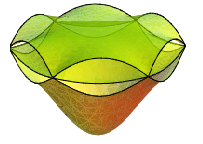
\includegraphics{diagrams/kagomeband.png}
\end{figure}
\ei 
\end{block}
}
\only<2>
{
On honeycomb lattice, no such band insulator. 
\bi 
\item Proposed wavefunction:
$$
\ket{\psi} = \prod\limits_R \sum\limits_{i \in R} b^{\dagger}_i \ket{\vec{0}}
$$
\item Goals:
\bi 
\item Rule out spontaneous symmetry breaking by computing correlations
\item Rule out topological order by computing topological entanglement entropy
\item Distinguish from other featureless phases using edge entanglement
\ei 
\ei 
}
\end{frame}
\subsection{Tensor Network Construction}
\begin{frame}{Tensor Network Construction of FBI}
\vskip-1.5cm
A wavefunction written as a product of local operators acting on a product state can simply be turned into a tensor network.


\note{Computations done by putting state on cylinder and using infinite-MPS techniques. Limited to circumference 10 cylinders by construction of transfer matrix.}
\end{frame}
\subsection{Entanglement Spectra Results}
\begin{frame}{Entanglement Spectra}
\vskip-1.5cm
\begin{figure}
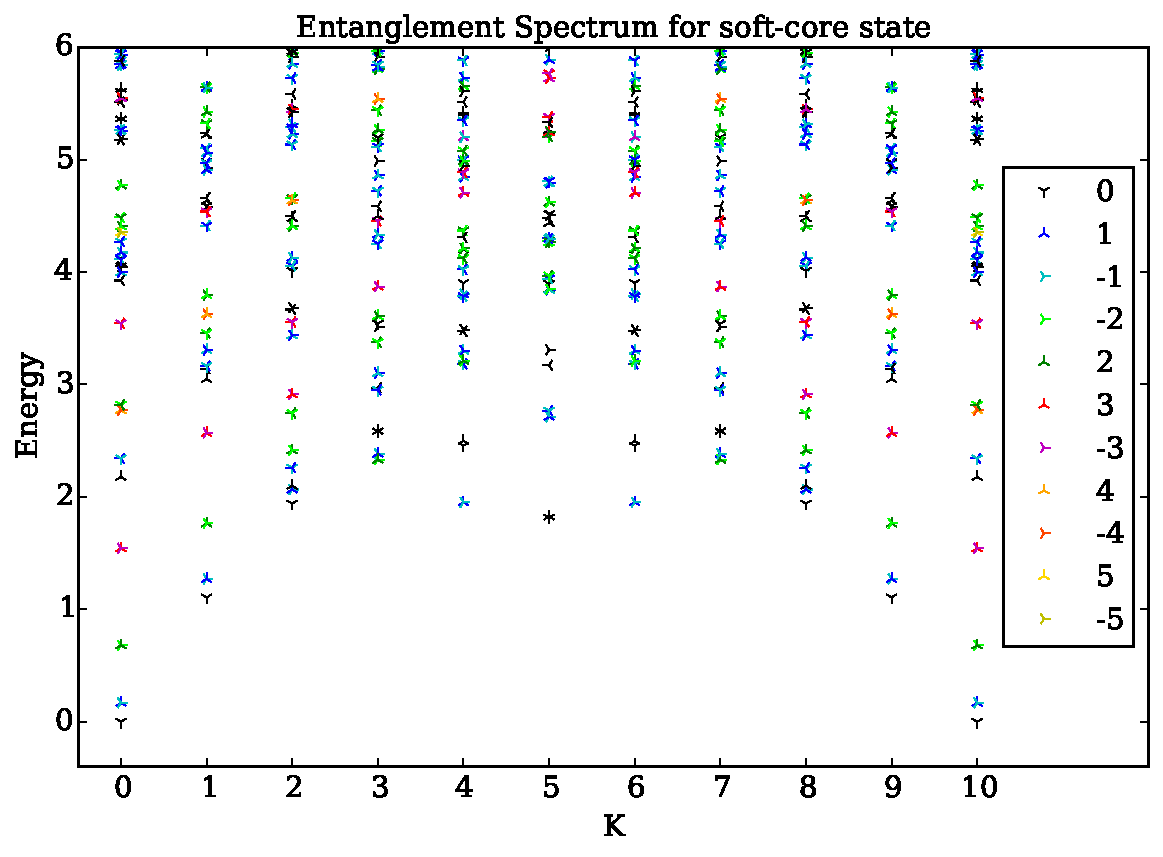
\includegraphics[width=\textwidth]{{interpolatedboson/new_plots/L_10_all_mom_10.pdf}}
\end{figure}
\end{frame}
\begin{frame}{Finite Size Analysis of Spectra}
\vskip-1.5cm
\begin{columns}[T]
    \begin{column}{.4\textwidth}
        \bi 
        \item<1-> Topological entanglement entropy is 0 
        \item<2-> Low energy modes show gapless $1/L$ behavior
        \ei
    \end{column}
    \begin{column}{.6\textwidth}
    \vskip-.3cm
        \only<2>{
        \begin{figure}[hbctp]
        \centering
        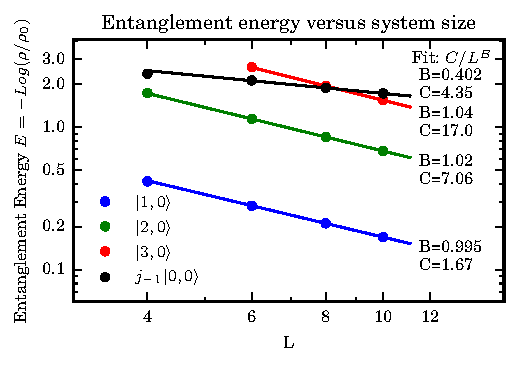
\includegraphics[width=2.5in]{{interpolatedboson/a10/plots/EntanglementEnergyScaling2.pdf}}
        %\caption{Power law fits for the lowest three states above the ground state at momentum zero and lowest two states at momentum 1 in Figure \ref{fig:sc-EEFinitesize}. The $1/L$ scaling is a signature of a gapless (entanglement) Hamiltonian. The labeling of the states $\ket{e, m}$ or $j_{-1} \ket{e, m}$ is explained in the CFT section below.}
        %\label{fig:sc-EEScaling}
        \end{figure}
        }
    \end{column}
\end{columns}
\end{frame}
\subsection{Identifying CFTs by Spectra}
\begin{frame}{Identifying CFTs: Measuring c}
\vskip-1.5cm
\begin{figure}[hbctp]
\centering
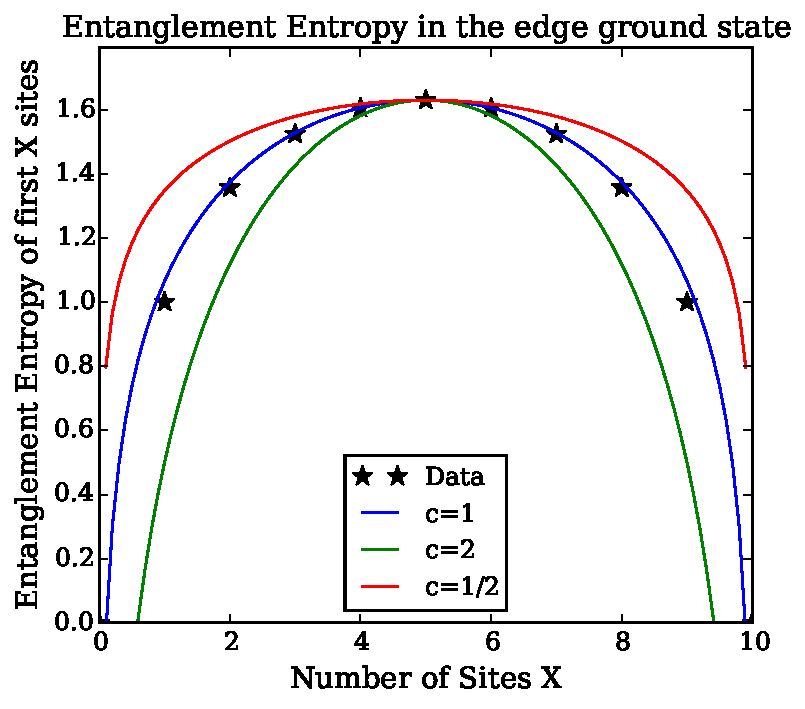
\includegraphics[height=\textheight]{{interpolatedboson/a0/plots/edge_gs_EE.pdf}}
\caption{Entanglement entropy within the entanglement ground state of the soft-core boson state on $10$ sites. For comparison, the Cardy-Calabrese formula $S(x) = c/3 \log \sin( \pi x/L) + const.$ is shown with $c=\frac{1}{2}, 1,$ and $2$, with the $const.$ fixed by matching the maximum of the entanglement entropy data. $c=1$ is a good fit.}
\label{fig:hc-edge-gs-ee}
\end{figure}
\end{frame}
\newcommand{\uL}{\mathbf{L_0}}
\newcommand{\bL}{\mathbf{\bar{L}_0}}
\begin{frame}{Level identification in CFT spectra}
\vskip-1.5cm
\only<1>{

To make a precise comparison with the free-boson CFT, we'll need to solve for (or look up) the solution of this model.

The free-boson CFT is created from the Lagrangian 
$$ \mathfrak{L} = \frac{g}{2}\int dt \int\limits_0^L dx ( \frac{1}{v^2}(\partial_t \phi)^2 - (\partial_x \phi)^2)$$
and with the compatified field identification
$$ \phi \equiv \phi + 2\pi R$$
and placed on the circle of circumference $L$ with periodic boundary conditions
$$ \phi(x) \equiv \phi(x+L).$$
}
\only<2>{
\begin{table}[h]
\centering
\begin{tabular}{c|c}
$\uL$ & $2\pi g(\frac{e}{4 \pi g R} + \frac{m R}{2})^2 + n$  \\
& \\
$\bL$ & $2\pi g(\frac{e}{4 \pi g R} - \frac{m R}{2})^2 + \bar{n}$  \\
& \\
$\mathbf{P} =\frac{2\pi v}{L}(\uL-\bL)$ & $\frac{2\pi v}{L}(em + n - \bar{n})$ \\
& \\
$\mathbf{H} = \frac{2\pi v}{L}(\uL+\bL)$ & $\frac{2\pi v}{L}(\frac{e^2}{4 \pi g R^2} + \pi g m^2 R^2 + n + \bar{n})$ \\
& \\
$\tilde{\mathbf{H}} = \frac{L}{2 \pi v \kappa}\mathbf{H}$ & $e^2 + \frac{m^2}{4 \kappa^2} + \frac{1}{\kappa}(n + \bar{n})$       
\end{tabular}
\label{Table:EV}
\caption{Eigenvalues of states $\ket{e, m}_{n, \bar{n}}$. The rescaled Hamiltonian $\tilde{\mathbf{H}}$ has eigenvalues that depend on only one free-parameter, $\kappa = 1/(4 \pi g R^2)$.(Note: A common convention is to set $g=1/4\pi$ and describe the system using $R=\sqrt{1/\kappa}$.) }
\end{table}
}
\only<3->{
\begin{figure}[hbctp]
\begin{center}
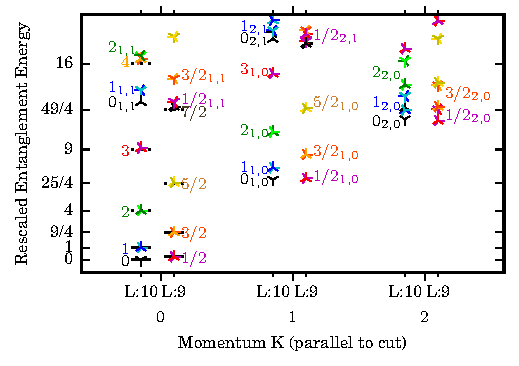
\includegraphics[height=\textheight]{{interpolatedboson/a10/plots/EEIdentify.pdf}}
\end{center}
%\caption{The identification of the states $\ket{e, m}_{n, \bar{n}}$ in the spectrum of the soft-core boson entanglement Hamiltonian. The label $e$ gives the U(1) charge. The labels $n$, $\bar{n}$ label the levels in the right or left-moving sectors of the Kac-Moody algebra. When the level $n$ is larger than 1, the level shows $Z(n)$ approximately degenerate states. The best estimate for the Luttinger parameter $\kappa = 1/6.4$ is given by the inverse of the energy of the $\ket{1, 0}_{1, 0}$ state. The label $m$ is 0 for all states shown - however, the primary states $\ket{e, m=\pm 1}$ can be seen centered around momentum $\pi$, with energies on the order of $1/(4\kappa^2)$.}
%\label{fig:primaries}
\end{figure}
}  
\end{frame}
\subsection{Open Questions and Speculations}
%\begin{frame}{Open questions and speculation}
Correspondence between edge and bulk physics
In a RG-fixed point tensor network state (such as toric code):
Can 
\end{frame}
\section*{}

%\frame{
  \vspace{2cm}
  {\huge Questions?}

  \vspace{3cm}
  \begin{flushright}
    Brayden Ware

    \structure{\footnotesize{brayden@physics.ucsb.edu}}
  \end{flushright}
}

\frame{
  \vfill
  \centering
  \highlighton{
  \usebeamerfont*{frametitle}Bonus slides

  %\usebeamerfont*{framesubtitle}Bonus slides
  }
  \vfill
}

\begin{frame}
  \frametitle{Resources}
  \vskip-1.7cm
  %\framesubtitle{If you want to improve this style}
  \bibliography{references}
  %\beamertemplatearticlebibitems
\end{frame}



\end{document}
